%% Springer Nature (sn-jnl, Sürüm 3.1) şablonu, iki sütun — Machine Vision and Applications sürümü (mva-tr).
%% Derleme: latexmk -pdf main.tex; latexmk -pdf ek.tex; latexmk -pdf main.tex (çapraz atıflar xr-hyper ile)
%% xr-hyper, hyperref'ten önce yüklenmelidir; sn-jnl.cls hyperref'i sınıf içinde yüklediğinden \documentclass'tan önce gelir.
\RequirePackage{xr-hyper}
\documentclass[pdflatex,iicol,sn-mathphys-num]{sn-jnl}

\usepackage[utf8]{inputenc}
\usepackage[T1]{fontenc}
\usepackage{lmodern}
\usepackage[protrusion=true,expansion=true]{microtype}
\usepackage[english,turkish,shorthands=off]{babel}
\usepackage{graphicx}
\usepackage{amsmath,amssymb,amsfonts}
\usepackage{amsthm}
\usepackage{booktabs,array,tabularx}
\usepackage{xcolor}
\usepackage{placeins}
\usepackage[title]{appendix}
\usepackage{pgfplots}
\usepackage{pgfplotstable}
\pgfplotsset{compat=1.18}
\usetikzlibrary{arrows.meta,calc,positioning,shapes.geometric,fit,backgrounds}
\usepgfplotslibrary{groupplots}
\definecolor{iyiRenk}{RGB}{0,84,159}
\definecolor{kotuRenk}{RGB}{178,24,43}
\providecommand{\iyi}[1]{\textcolor{iyiRenk}{\textbf{#1}}}
\providecommand{\kotu}[1]{\textcolor{kotuRenk}{\textit{#1}}}
\newcolumntype{Y}{>{\centering\arraybackslash}X}
\providecommand{\figroot}{figures/}
\newcommand{\burl}[1]{\url{#1}}
% İngilizce başlık, özet ve anahtar kelimeler (Türkçe özetin altında, başlık sayfasında)
\newcommand{\ingilizceblok}[3]{\par\medskip
  \begin{otherlanguage*}{english}%
  \noindent\textbf{Title:} #1\par\medskip
  \noindent\textbf{Abstract.} #2\par\medskip
  \noindent\textbf{Keywords:} #3%
  \end{otherlanguage*}}

\raggedbottom
\makeatletter\def\keywordname{Anahtar Kelimeler}\makeatother
\hypersetup{hypertexnames=false}
\externaldocument{ek}% genişletilmiş ek (paper/ek.pdf) atıfları

\begin{document}

\title[YOLO İnce Ayarında Çok Tohumlu Değerlendirme: VOC ve KITTI]{Gerçek Zamanlı YOLO Modellerinin İnce Ayarında Artırma ve Kayıp Müdahalelerinin Çok Tohumlu Değerlendirmesi: PASCAL VOC ve KITTI Üzerine Bir İnceleme}

%% Yazarlar (danışman kararı, 2026-10-18): 1. ve sorumlu yazar öğrenci; 2. yazar danışman
\author*[1]{\fnm{Ahmed Gürkan} \sur{ÖZÇELİK}}\email{250801017@ostimteknik.edu.tr}
\author[1]{\fnm{Ufuk} \sur{ASIL}}\email{ufuk.asil@ostimteknik.edu.tr}
\affil*[1]{\orgname{Ostim Technical University},
  \orgaddress{\street{OSTİM, 100. Yıl Bulvarı, 55/F}, \postcode{06374},
  \city{Yenimahalle}, \state{Ankara}, \country{Türkiye}}}

\abstract{Bu çalışmada, gerçek zamanlı nesne tespit modellerinin ince ayarında veri artırma ve kayıp değişikliklerinden koşumdan önce beklenen kazanç birkaç onda bir puandı ve eğitim tohumuna bağlı oynaklıkla aynı büyüklükteydi. Sorumuz, böyle küçük kazanç iddialarının tipik bir üç tohumlu ince ayar bütçesinde gürültüden ayrılıp ayrılamadığı ve ayrılamıyorsa gürültünün nereden geldiğidir. Taban modelden (baseline) yalnız bir ayarla ayrılan yedi eğitim-zamanı müdahalesini ve eğitimsiz çıkarım seçeneklerini COCO ön-eğitimli YOLO11n ile PASCAL VOC 07+12'de, YOLO11s ve YOLO26n ile KITTI'de değerlendirdik. Ön-kayıt esaslı protokolde kabul kararları üç tohumla verildi, test kümeleri müdahaleler için kilitli tutulup bir kez açıldı ve eşikler koşumdan önce sabitlendi. Bu tasarım VOC doğrulamasında yalnız $\gtrsim$1 puanlık etkileri güvenle ayırabilir; KITTI'de kritik etki 2.92 ile 3.61 puan arasındadır. VOC'ta yedi müdahalenin hiçbiri doğrulamada kabul eşiğini geçmedi (0/7). Kilit sonrası, önceden yazılmış ölçütlerle yapılan bir bileşen analizinde ayarsız Varifocal kaybındaki düşüş esas olarak negatif örneklerin bastırılmasına bağlandı; keşifsel bir telafi kartında sınıflandırma kaybı kazancı düşüşün $\approx$\%82'sini geri kazandırdı. KITTI'de on iyileşme sınamasından yalnız biri eşiği geçti (1/10); bu kabul son epoch ağırlıklarıyla işaret değiştirdi ve kazancın çoğu tek bir test sahne grubundan geldi, bu yüzden KITTI'yi genelleme kanıtı saymıyoruz. Sonuçlar, ayarlanmamış varsayılan reçeteye karşı ayarsız tek noktalı müdahaleler için geçerlidir. Küçük kazanç iddiaları bu bütçede gürültüden ayrılamadı; çalışma gürültünün dört kaynağını belgeler: tohum varyansı, doğrulama örneklemesi, tek tohumlu ön-eleme ve kontrol noktası seçimi. Katkı yöntemseldir ve kapsamı dardır.
\par\medskip\noindent\textbf{Anahtar Kelimeler:} nesne tespiti, YOLO, ince ayar, tekrarlanabilirlik, tohum varyansı, negatif sonuçlar}

\maketitle

{\small\ingilizceblok{A Multi-Seed Evaluation of Augmentation and Loss Interventions in Fine-Tuning Real-Time YOLO Detectors: A Study on PASCAL VOC and KITTI}{Gains expected from augmentation and loss changes in fine-tuning real-time detectors were a few tenths of a point, the same order as seed-to-seed variation. We ask whether such small-gain claims can be separated from noise under a typical three-seed fine-tuning budget and, if not, where the noise comes from. Seven training-time interventions and training-free inference options, each changing one baseline setting, were evaluated with COCO-pretrained YOLO11n on PASCAL VOC 07+12 and with YOLO11s and YOLO26n on KITTI. The pre-registration-based protocol uses three seeds per acceptance decision, test sets locked for the interventions and opened once, and thresholds fixed before the runs. The design resolves only effects of $\gtrsim$1 point on VOC validation; on KITTI the critical effect is 2.92 to 3.61 points. On VOC, none of the seven interventions met the acceptance threshold on validation (0/7). A post-lock component analysis against pre-written criteria traced the drop under untuned Varifocal loss mainly to the suppression of negative samples; in an exploratory run, compensating the classification loss gain recovered $\approx$82\% of the drop. On KITTI, one of ten improvement tests passed (1/10); it reversed sign with last-epoch weights and most of the gain came from a single test scene group, so we do not read KITTI as evidence of generalization. The results hold for untuned single-point interventions against an untuned default recipe. Such claims were not separable from noise here; the paper documents four noise sources: seed variance, validation sampling, single-seed screening and checkpoint selection. The contribution is methodological and narrow.}{object detection; YOLO; fine-tuning; reproducibility; seed variance; negative results}\par}

\section{Giriş}\label{sec:giris}

Gerçek zamanlı nesne tespiti, gecikme bütçesi milisaniyelerle ölçülen uygulamalarda ve donanımı kısıtlı cihazlarda kullanılır; bu alanın başlıca araçlarından biri tek geçişli YOLO (You Only Look Once) ailesidir \cite{redmon_2016_yolo,jocher_2024_yolo11}. Bu ailede mimari sabit tutularak yalnız eğitim reçetesi değiştirilebilir: bir veri artırma biçimi, bir kutu kaybı ya da bir son işlem adımı eklenir ve doğruluk tablosunda küçük bir artış görülür. Böyle küçük bir artışın ne kadarının gerçek, ne kadarının eğitim tohumunun ve model seçiminin ürünü olduğu tek koşumluk bir karşılaştırmada ayırt edilemez. Makine öğrenmesinin başka alanlarında iyileştirme iddialarının doğru ayarlı bir taban modele (baseline) ve varyans hesabına karşı sınanmadığı gösterilmiştir \cite{lipton_2019_troubling}. PASCAL VOC için resmî Ultralytics yapılandırmasında en iyi kontrol noktasının (eğitim sırasında doğrulama ölçütüne göre saklanan ağırlık, \texttt{best.pt}) VOC07 test kümesinde seçildiği ise bir çalışmada açıkça kabul edilmiştir \cite{lin_2026_yolopeft}.

Pratikte sık görülen rejimde ön-eğitimli küçük bir ağırlık hedef veriye ince ayarlanır. Veri artırma ve kayıp ayarları çıkarım grafiğine dokunmadığından en ucuz kaldıraç gibi görünür, ama beklenen kazanç ile gürültü aynı büyüklüktedir: COCO ön-eğitimli YOLO11n'in PASCAL VOC 07+12 ince ayarında üç tohumlu taban modelin doğrulama ortalama kesinlik ortalaması (mean average precision, mAP; burada mAP50-95) standart sapması 0.41 puandır, müdahalelerden koşumdan önce beklenen fark ise birkaç onda birdir. Soru şudur: küçük kazanç iddiaları tipik bir ince ayar bütçesinde gürültüden ayrılabilir mi, ayrılamıyorsa gürültünün kaynakları nelerdir?
Önerilen teknikler çoğunlukla başka bir model ölçeğinde, veri kümesinde ve uzun eğitimde değerlendirilmiştir (ör. maskeli Copy-Paste büyük modellerle \cite{ghiasi_2021_copypaste}; YOLOX'un küçük modellerde zayıf artırma önerisi \cite{ge_2021_yolox}); kutu etiketli, nano ölçekli kısa bir ince ayara aktarımları varsayılamaz. Tekrarlanabilirlik literatürü gerekli araçları sağlar \cite{bouthillier_2021_variance,picard_2021_seed}, ancak bu araçların gerçek zamanlı tespit ince ayarına çok tohumlu, kilitli test kümeli ve önceden yazılmış karar kurallarıyla uygulandığı bir çalışma incelediğimiz kaynaklarda bulunamadı (tarama kapsamı: Bölüm~\ref{sec:ilgili}).
Bu çalışma yeni bir dedektör önermez; küçük iyileştirmeleri sınamak için uyguladığımız ön-kayıt esaslı protokolü ve sonuçlarını raporlar. Her müdahale taban modelden tek bir ayarla ayrılır ve koşumdan önce sabitlenen eşiklerle karara bağlanır; müdahaleler yalnız doğrulama kümesinde seçilir ve test kümesi seçim bittikten sonra bir kez kullanılır. Karşılaştırma, ayarlanmamış varsayılan reçeteye karşı ayarsız tek noktalı müdahalelerdir. Kilitli test açıldıktan sonra eklenen koşumlar ve önceden yazılmış kurallardan sapmalar ayrıca beyan edilmiştir (Bölüm~\ref{sec:cerceve} ve \ref{sec:sinirliliklar}). Merkez tezimiz şudur: Küçük kazanç iddiaları tipik bir üç tohumlu ince ayar bütçesinde gürültüden ayrılamadı; makale bunu yedi müdahale ve iki veri kümesiyle gösterir ve gürültünün dört kaynağını belgeler: tohum varyansı, doğrulama örneklemesi, tek tohumlu ön-eleme ve kontrol noktası seçimi.

VOC'ta yedi eğitim-zamanı müdahalesinin hiçbiri üç tohumlu doğrulamada kabul eşiğini geçmedi (0/7); kilitli teste giren tek eğitim müdahalesi olan kutu-tabanlı copy-paste (H03) doğrulamada +0.25 puan önde iken testte $-$0.12 puan geride kaldı. KITTI'de YOLO11s ve YOLO26n'in on iyileşme sınamasından yalnız biri, YOLO11s'te çok ölçekli eğitim (H01), eşiği geçti; bu kabul son epoch ağırlığı (\texttt{last.pt}) kullanıldığında işaret değiştirir ve kazancının çoğu tek bir test sahne grubundan gelir. KITTI deneyini bu yüzden bir genelleme kanıtı olarak değil, kontrol noktası seçim gürültüsünün bir gösterimi olarak okuyoruz. Katkılar şunlardır: (i) yedi eğitim-zamanı müdahalesi ve eğitimsiz çıkarım seçenekleri, gecikmeleriyle, çok tohumlu, kilitli test kümeli ve önceden yazılmış karar kurallarına bağlı bir protokolle değerlendirildi; (ii) küçük farklara dayanan iddialardaki dört gürültü kaynağı belgelendi ve her biri için pratik bir öneri türetildi (Bölüm~\ref{sec:gurultu}); (iii) ayarsız Varifocal kaybıyla görülen düşüş bileşenlerine ayrıldı.

Deney kaydının özeti ve hesap notları Ek~\ref{sec:deney-kaydi}'dadır; ek sonuçlar ve yöntem ayrıntıları genişletilmiş ektedir (GitHub deposu, \texttt{paper/ek.pdf}) ve makale bu belgeye ``genişletilmiş ek, Bölüm X.n'' biçiminde atıf yapar.

\section{İlgili Çalışmalar}\label{sec:ilgili}

\paragraph{Gerçek zamanlı tespit.}
YOLO ailesi tespiti tek geçişli bir regresyon problemi olarak kuran YOLOv1 ile başlamıştır \cite{redmon_2016_yolo}. Sonraki sürümler mimariden çok eğitim reçetesini zenginleştirmiştir; örneğin YOLOX ayrık başlığı ve çapasız tasarımı getirmiştir \cite{ge_2021_yolox}. YOLO11 hakemli bir teknik raporla belgelenmemiş bir Ultralytics sürümüdür \cite{jocher_2024_yolo11}; YOLO26 raporu maksimum olmayanı bastırma (non-maximum suppression, NMS) gerektirmeyen uçtan uca çıkarımı ve MuSGD optimizatörünü tanıtır \cite{jocher_2026_yolo26}; taban modelimiz MuSGD'yi paket varsayılanı olarak devralır. Odağımız mimari değil, küçük YOLO modellerinin eğitim ve çıkarım ayarlarıdır.

\paragraph{Veri artırma ve kayıp fonksiyonları.}
Mosaic dört görüntüyü tek örnekte birleştirir; YOLOX küçük modellerde güçlü artırmanın, iki görüntüyü harmanlayan MixUp dahil, zayıflatılmasını önerir \cite{ge_2021_yolox}. Nesne kesip yapıştırma fikri Cut-Paste-Learn'e dayanır \cite{dwibedi_2017_cutpaste}; Ghiasi ve ark. bunu bölütleme maskeleriyle, COCO'da büyük modeller ve uzun eğitimle güçlü bir artırma olarak gösterir \cite{ghiasi_2021_copypaste}, Kisantal ve ark. küçük nesneleri çoğaltarak yapıştırır \cite{kisantal_2019_smallaug}. Ultralytics'in yerleşik \texttt{copy\_paste} artırması bölütleme içindir ve varsayılan olarak kapalıdır \cite{ultralytics_2026_v84165}. Kutu regresyonunda DIoU ve tam IoU (complete IoU, CIoU) merkez uzaklığı ve en-boy terimleri ekler \cite{zheng_2020_diou}; Inner-IoU yardımcı kutularla bu çizgiyi sürdürür \cite{zhang_2023_inneriou}. CIoU Ultralytics'in varsayılan kutu kaybıdır \cite{ultralytics_2026_v84165}; ``CIoU'ya geçiş'' türü kazançlar taban modelimizde zaten bulunur. VarifocalNet sınıf hedefini IoU ile ölçekleyen Varifocal Loss'u (VFL) \cite{zhang_2021_varifocalnet}, GFL kalite odaklı sınıflandırmayı ve dağılım odaklı kutu kaybını (DFL) önerir \cite{li_2020_gfl}. TOOD'un görev-hizalı atayıcısı (TAL) sınıf skoru ile IoU'yu birlikte kullanır \cite{feng_2021_tood}; PP-YOLOE VFL'yi TAL ile standart reçetesine aldığından bu ikilinin tek başına zararlı olması beklenmez \cite{xu_2022_ppyoloe}.

\paragraph{Çıkarım zamanı işlemleri ve küçük nesneler.}
Soft-NMS örtüşen kutuları silmek yerine skorlarını düşürür \cite{bodla_2017_softnms}; DIoU-NMS bastırma ölçütüne merkez uzaklığını katar \cite{zheng_2020_diou}. Ağırlıklı kutu füzyonu (weighted boxes fusion, WBF) farklı modellerin kutularını birleştirmek için tasarlanmıştır \cite{solovyev_2021_wbf}; tek modelde kullanımı ayrıca sınanmalıdır. Test-zamanı artırma (test-time augmentation, TTA) çıkarım çözünürlüğünü de değiştirdiğinden kazancı artırmanın kendisinden ayırmak güçtür \cite{ultralytics_2026_yolov5tta}. Bu yöntemlerin çoğu gerçek-zaman gecikme kısıtı altında değerlendirilmemiştir; biz onları önceden belirlenmiş göreli bir gecikme bütçesiyle tek model için sınarız. Küçük nesne açığı için küçük nesne odaklı artırma önerilmiştir \cite{kisantal_2019_smallaug}.

\paragraph{Tekrarlanabilirlik, tohum varyansı ve boşluk.}
Lipton ve Steinhardt iyileşmenin gerçek kaynağını bulandıran eğilimleri sıralar \cite{lipton_2019_troubling}. Picard tohum varyansı mütevazı olsa da aykırı tohum bulmanın kolay olduğunu gösterir \cite{picard_2021_seed}; Bouthillier ve ark. varyans kaynaklarını hesaba katan bir karşılaştırma protokolü önerir \cite{bouthillier_2021_variance}; Cawley ve Talbot seçim ölçütüne aşırı uyumun performans tahminini şişirebileceğini gösterir \cite{cawley_2010_overfitting}. Kararları sonuçtan önce yazma fikrini ön-kayıt uygulamasından ödünç alırız \cite{nosek_2018_preregistration}. v8.4.165 varsayılanlarının hangi veriyle ayarlandığına dair resmî bir belge bulamadık; COCO'da ayarlı oldukları bir varsayımdır. YOLO-PEFT, resmî VOC yapılandırmasını izleyen sonuçlarının tek açılışlı kör test tahmini olmadığını kabul eder \cite{lin_2026_yolopeft}; bu yapılandırmayı izleyen VOC sonuçları iyimser olabilir ve çıpa olarak kullandığımız diğer kaynaklar için bu durum doğrulanamadı (Bölüm~\ref{sec:replikasyon}).

İncelediğimiz kaynaklarda, gerçek zamanlı tespitte bir müdahaleyi doğrulanmış bir taban modele karşı çok tohumlu, kilitli bir test kümesi (tek açılış) ve önceden yazılmış karar kurallarıyla sınayan bir çalışma bulamadık; bu bir yokluk iddiası değildir, aşağıda verilen taramanın kapsamını yansıtır. Tarama sistematik değildir: kaynaklar Crossref, arXiv, Semantic Scholar API, yayıncı sayfaları ve web aramasıyla bulunup doğrulandı; ana tarama 2026-09-29 ile 2026-10-02 arasında yapıldı, KITTI deneyi ve sonraki analizlerle ilgili üç kaynak sonradan (2026-10-03 ile 2026-10-22 arasında) eklendi ve arama sorguları kaydedilmedi.

\section{Yöntem}\label{sec:yontem}

{\tikzset{every picture/.append style={yscale=0.75}}% yalnız görsel yükseklik
% F0 -- önceden yazılmış karar kurallarıyla protokol akışı (şematik; veri içermez). Şekil içi metin ve başlık Türkçe.
\begin{figure*}[t]
\centering
\resizebox{\textwidth}{!}{%
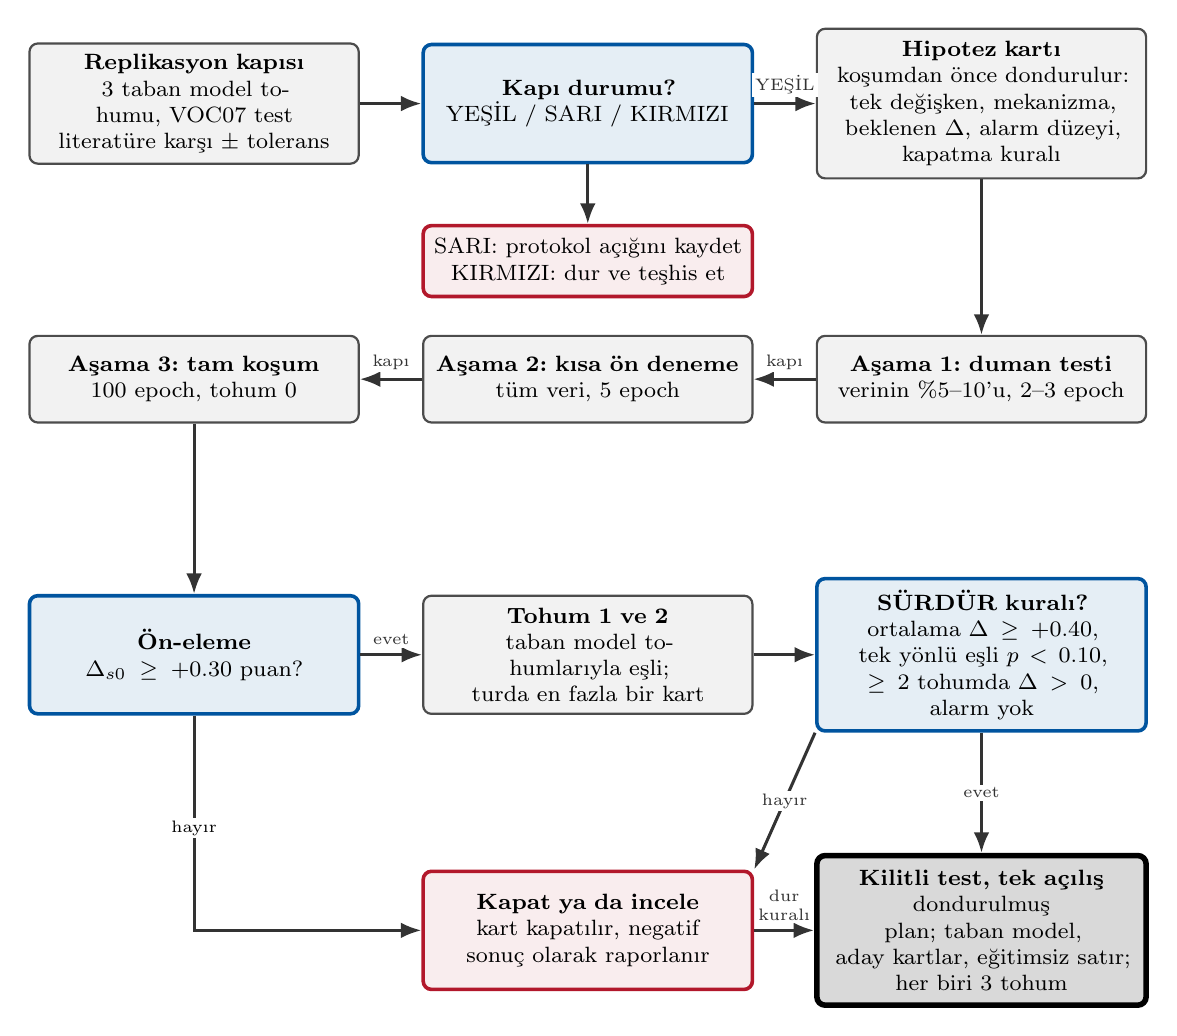
\begin{tikzpicture}[
  box/.style={rectangle, rounded corners=3pt, draw=black!70, fill=black!5, line width=0.8pt,
    align=center, text width=3.9cm, minimum height=1.1cm, inner sep=4pt, font=\footnotesize},
  gate/.style={box, draw=iyiRenk, fill=iyiRenk!10, line width=1.3pt},
  stop/.style={box, draw=kotuRenk, fill=kotuRenk!8, line width=1.3pt},
  lock/.style={box, draw=black, fill=black!15, line width=2pt},
  arr/.style={-{Latex[length=2.6mm,width=2mm]}, line width=1.1pt, black!80},
  lab/.style={font=\fontsize{6}{7}\selectfont, fill=white, inner sep=1pt, align=center}
]
% ---- satır 1: taban model geçerliliği ve kart
\node[box,  minimum height=1.5cm] (A) at (0,0)    {\textbf{Replikasyon kapısı}\\3 taban model tohumu, VOC07 test\\literatüre karşı $\pm$ tolerans};
\node[gate, minimum height=1.5cm] (B) at (5.0,0)  {\textbf{Kapı durumu?}\\YEŞİL / SARI / KIRMIZI};
\node[box,  minimum height=1.9cm] (C) at (10.0,0) {\textbf{Hipotez kartı}\\koşumdan önce dondurulur:\\tek değişken, mekanizma,\\beklenen $\Delta$, alarm düzeyi,\\kapatma kuralı};
\node[stop, minimum height=0.9cm] (S) at (5.0,-2.0) {SARI: protokol açığını kaydet\\KIRMIZI: dur ve teşhis et};
% ---- satır 2: aşamalı koşum (sağdan sola)
\node[box] (D) at (10.0,-3.5) {\textbf{Aşama 1: duman testi}\\verinin \%5--10'u, 2--3 epoch};
\node[box] (E) at (5.0,-3.5)  {\textbf{Aşama 2: kısa ön deneme}\\tüm veri, 5 epoch};
\node[box] (F) at (0,-3.5)    {\textbf{Aşama 3: tam koşum}\\100 epoch, tohum 0};
% ---- satır 3: kararlar
\node[gate, minimum height=1.5cm] (G) at (0,-7.0)    {\textbf{Ön-eleme}\\$\Delta_{s0}\ge+0.30$ puan?};
\node[box,  minimum height=1.5cm] (H) at (5.0,-7.0)  {\textbf{Tohum 1 ve 2}\\taban model tohumlarıyla eşli;\\turda en fazla bir kart};
\node[gate, minimum height=1.9cm] (I) at (10.0,-7.0) {\textbf{SÜRDÜR kuralı?}\\ortalama $\Delta\ge+0.40$,\\tek yönlü eşli $p<0.10$,\\$\ge2$ tohumda $\Delta>0$,\\alarm yok};
% ---- satır 4: sonuçlar
\node[stop, minimum height=1.5cm] (K) at (5.0,-10.5)  {\textbf{Kapat ya da incele}\\kart kapatılır, negatif\\sonuç olarak raporlanır};
\node[lock, minimum height=1.9cm] (J) at (10.0,-10.5) {\textbf{Kilitli test, tek açılış}\\dondurulmuş plan; taban model,\\aday kartlar, eğitimsiz satır;\\her biri 3 tohum};
% ---- oklar
\draw[arr] (A) -- (B);
\draw[arr] (B) -- (C) node[lab, pos=0.5, above=2pt] {YEŞİL};
\draw[arr] (B) -- (S);
\draw[arr] (C) -- (D);
\draw[arr] (D) -- (E) node[lab, pos=0.5, above=2pt] {kapı};
\draw[arr] (E) -- (F) node[lab, pos=0.5, above=2pt] {kapı};
\draw[arr] (F) -- (G);
\draw[arr] (G) -- (H) node[lab, pos=0.5, above=2pt] {evet};
\draw[arr] (H) -- (I);
\draw[arr] (G.south) |- (K.west);
\node[lab] at (0,-9.2) {hayır};
\draw[arr] (I.south west) -- (K.north east) node[lab, pos=0.5] {hayır};
\draw[arr] (I) -- (J) node[lab, pos=0.5] {evet};
\draw[arr] (K) -- (J) node[lab, pos=0.5, above=2pt, align=center] {dur\\kuralı};
\end{tikzpicture}}%
\caption{Önceden yazılmış karar kurallarıyla analiz protokolünün akışı. Mavi çerçeveli kutular karar kapısı (koşumdan önce yazılmış), kırmızılar durdurma veya kart kapanışı, kalın çerçeve kilitli testtir.}\label{fig:f0-protokol}
\end{figure*}
}

İnce ayar rejiminde bir müdahaleden beklenen kazanç eğitim tohumunun oynaklığıyla aynı büyüklüktedir; kararı sonuçlara bakarak vermek bu koşulda seçilim yanlılığına yol açabilir \cite{cawley_2010_overfitting,bouthillier_2021_variance}. Protokol bu nedenle kararı koşumdan önce sabitler \cite{nosek_2018_preregistration}: hipotez ve eşikler yazılır, taban model doğrulanır, koşumlar kademelendirilir ve test kümesi bir kez açılır (Şekil~\ref{fig:f0-protokol}). Kurallar, bir istisna dışında koşumdan önce yazılmıştır: SÜRDÜR kuralı tur 2'de, H01--H03 sonuçlarından sonra donmuştur (Bölüm~\ref{sec:karar}). Kamuya açık, zaman damgalı bir kayıt ise yoktur; ayrıntı Sınırlılıklar'dadır (Bölüm~\ref{sec:sinirliliklar}).

\subsection{Önceden yazılmış karar kurallarıyla analiz çerçevesi}\label{sec:cerceve}

Doğruluk değerleri puan cinsindendir (mAP$\times100$). $M_{c,s}$, $c$ yapılandırmasının $s$ tohumuyla eğitilmiş modelinin doğrulama mAP50-95 değeridir (IoU eşiği 0.50'den 0.95'e 0.05 adımla). $B$ taban modeli, $k$ bir müdahale kartını, $S=\{0,1,2\}$ tohum kümesini temsil eder; $n=|S|=3$. Aynı tohumla eşleştirilmiş fark ve ortalaması
\begin{equation}\label{eq:delta}
\Delta_{k,s}=M_{k,s}-M_{B,s},\qquad \bar\Delta_k=\frac1n\sum_{s\in S}\Delta_{k,s}
\end{equation}
olarak tanımlanır.

\paragraph{Hipotez kartı.}
Her müdahale koşumdan önce yazılan bir hipotez kartıyla (hypothesis card) tanımlanır. Kart tek değişkeni, mekanizmayı, beklenen yön ve büyüklüğü, ``görülmemiş iyi'' sayılacak kırmızı bayrak eşiğini, kapatma kuralını, bütçeyi ve ikincil metrikleri sabitler; kartın üst kısmı sonradan değişmez ve düzeltme yeni kartla yapılır (bu kuralın uygulamadaki kanıt gücü sınırlıdır; Bölüm~\ref{sec:sinirliliklar}; kart kuralının tamamı: genişletilmiş ek, Bölüm~\ref{sec:ek-kart}). Kırmızı bayrak aşılırsa kart kabul edilmez ve sızıntı, bölme ve taban model denetlenir. Karar etiketleri SÜRDÜR (kart kabul edilir), KAPAT (kart kapanır) ve İNCELE'dir (ek inceleme gerekir).\footnote{Çalışmanın kayıtlarındaki özgün etiketler sırasıyla TUT, ÖLDÜR ve İNCELE'dir; metinde anlamları değiştirilmeden SÜRDÜR, KAPAT ve İNCELE olarak verilir.} Sekiz kartın değişkeni ve önceden yazılmış beklentisi Tablo~\ref{tab:kartlar}'dedir; aralıklar literatürden ya da en yakın çıpadan türetilmiştir.

\begin{table*}[t]
\centering\footnotesize\setlength{\tabcolsep}{4pt}
\caption{Sekiz hipotez kartı. Beklenen $\Delta$ ve kırmızı bayrak, doğrulama mAP50-95 farkının koşumdan önce yazılmış değerleridir [puan]; H07'de değerler satır ailesine göre değişir.}\label{tab:kartlar}
\begin{tabularx}{\textwidth}{@{}l l >{\raggedright\arraybackslash}X c c@{}}
\toprule
Kart & Aile & Taban modelden değişen tek şey & Beklenen $\Delta$ & Kırmızı bayrak \\
\midrule
H01 & Ölçek & batch çözünürlük aralığı $m$: $0\to0.25$ & $[0,\,{+}0.5]$ & $>{+}1.0$ \\
H02 & Kutu kaybı & CIoU $\to$ Inner-CIoU, $r=0.75$ & $[0,\,{+}0.5]$ & $>{+}1.0$ \\
H03 & Copy-paste & kutu-tabanlı, $p=0.5$, $\sqrt A\le48$ px & $[0,\,{+}0.4]$ & $>{+}0.8$ \\
H04 & Ölçek & görüntü-içi ölçek genliği $\sigma_s$: $0.5\to0.25$ & $[0,\,{+}0.5]$ & $>{+}1.0$ \\
H05 & Sınıf kaybı & BCE $\to$ Varifocal, $\alpha=0.75$, $\gamma=2$ & $[{-}0.5,\,{+}0.5]$ & $>{+}1.0$ \\
H06 & Kutu kaybı & kutu kazancı $\lambda_{\mathrm{box}}$: $7.5\to10$ & $[{-}0.3,\,{+}0.3]$ & $>{+}0.8$ \\
H07 & Eğitimsiz çıkarım & NMS eşiği, Soft-NMS, test çözünürlüğü, TTA, WBF (12 satır) & aileye göre $[0,\,{+}1.0]$ & $>{+}1.0\ldots{+}2.0$ \\
H08 & Copy-paste doz & $p=1.0$, $\sqrt A\le96$ px & $[0,\,{+}0.8]$ & $>{+}1.0$ \\
\bottomrule
\addlinespace[3pt]
\multicolumn{5}{@{}p{\dimexpr\textwidth-2\tabcolsep\relax}@{}}{Tek-değişken istisnaları: H08 olasılık ve aday havuzunu birlikte değiştirir (Bölüm~\ref{sec:mudahaleler}); YOLO26n'de H02 ve H05 iki eğitim başlığına birlikte uygulanır (Bölüm~\ref{sec:genelleme-protokol}).} \\
\end{tabularx}
\end{table*}

\paragraph{Makullük kapısı ve kademeli koşum.}
Üç tohumlu taban modelin VOC07 testindeki mAP50-95 ve mAP50 değerleri benzer protokolle yayımlanmış bir aralıkla karşılaştırılır (Bölüm~\ref{sec:replikasyon}). YEŞİL sonuçta müdahale aşamasına geçilir, SARI sonuçta protokol farkı belgelenir, KIRMIZI sonuçta koşum durur; tolerans sonradan genişletilmez. Kapı yalnız taban modeli sınar; taban model böylece test kümesini bir kez görmüş olur ve değerleri kapı raporunda ve deney günlüğünde yazılı olarak görülür; bu beyan edilir. Uygulama hataları ucuz aşamalarda yakalanır: aşama 1 duman testidir (verinin yüzde 5--10'u, 2--3 epoch), aşama 2 kısa ön denemedir (tam veri, 5 epoch), aşama 3 tam eğitimdir (100 epoch). Her aşamadan sonra koşumdan önce yazılmış bir beklenti dosyası (metrik sınırları, varyant imzası, sayaç aralıkları) denetlenir; ihlalde kuyruk durur. Aşama 3'te canlı bir güvenlik kuralı NaN oluşunca ya da belirli bir epoch'ta doğrulama metriği alt sınırın altında kalınca koşumu keser. $\texttt{epochs}\le\texttt{close\_mosaic}$ iken Ultralytics mosaic'i baştan kapattığından H03 ve H08'in aşama 1--2 koşumları \texttt{close\_mosaic=0} ile, aynı ayarlı bir taban modele karşı yapılır.

\paragraph{Test kilidi.}
Müdahaleler yalnız doğrulama kümesinde seçilir; döngü boyunca metrik dosyalarında test anahtarı bulunmaz. Test kümesi müdahaleler için yalnız döngü sonundaki kilitli adımda (K5) açıldı: 2026-10-01 21:23:45. Taban model değerleri ise makullük kapısı için 2026-09-30'da ölçüldü ve görüldü (ilk ölçüm 10:16:22; çıpa dosyası 2026-09-29 22:21:13'te yazılmıştı): kapı raporu (16:10) ve deney günlüğü bu değerleri yazar, tohum 0'ın ilk satırları ise kapı raporundan önce, 10:40'ta bir analiz adımında planlanandan erken görüldü (Bölüm~\ref{sec:sinirliliklar}). Aynı ağırlıklar K5'te aynı değerleri verdi (Bölüm~\ref{sec:replikasyon}). Kayıtlara göre iki ölçüm arasında H04--H08 kartları yazıldı, SÜRDÜR kuralı dondu ve H05'in güvenlik eşiği yeniden kalibre edildi; kayıtlardaki yazım notları bunların yalnız doğrulama bilgisiyle yazıldığını belirtir, makullük kapısının aralığı ve toleransı değişmedi. Yorumumuz şudur: taban model test değerleri müdahalelerin etkisi hakkında bilgi taşımaz, yalnız taban modelin mutlak düzeyini verir; ilk ölçümden sonra yazılan H04--H08 kartları ve SÜRDÜR kuralı açısından risk bu bilgiyle sınırlıdır. K5 planı (koşumlar, karşılaştırmalar, istatistikler) test koşumlarından önce yazılmıştır; sonra test kümesinde yeni hipotez, eğitim ya da hiperparametre araması yapılmaz. Döngü bir kart SÜRDÜR alınca, ardışık iki turda en iyi eğitim kartının $\Delta$'sı $+0.30$'un altında kalınca ya da bütçe (75 grafik işlem birimi, GPU, saati planlanan, 90 saat tavan) veya tur sınırı (5) dolunca K5'e geçer. K5 koşumları eğitimsizdir: taban model, doğrulamada eşiğe en yakın kart (H03) ve eğitimsiz TTA satırı üçer tohumla (dokuz koşum) girer; diğer kartlar yalnız doğrulamada değerlendirilir. Kilit açıldıktan sonra VOC'ta yalnız doğrulamada yapılan ek işler (elenen altı kartın tohum 1--2 koşumları, WBF tanı ızgarası, güç analizleri, H05 mekanizma kartları) teste uygulanmadı; KAPAT etiketleri ek tohumlardan önce verilmiş ve değişmemiştir (tam liste: Ek~\ref{sec:ek-kilit}).

\paragraph{Uygulama denetimleri.}
Kod hataları şu denetimlerle aranmıştır: kayıp değişikliklerinde özdeşlik birim testleri (Inner-CIoU $r=1$ iken ve VFL $\alpha=1$, $\gamma=0$ iken negatif hücrelerde taban kayıpla birebir eşleşme), VFL pozitif dalının elle yazılmış bir uygulamaya karşı çift duyarlıklı gradyan denetimi, WBF birim testleri (8/8), YOLO26n'de yamaların iki eğitim başlığına uygulandığını sayan başlık sayacı, kademeli koşumların beklenti dosyaları ve otomatik sağlık kapıları. Revizyonlarda metindeki her sayının önceki sürümde de bulunduğu bir sayı bütünlüğü betiğiyle denetlendi; ajanların ürettiği kod, analiz ve metin yazarlarca denetlendi.

\subsection{Taban model ve müdahaleler}\label{sec:mudahaleler}\label{sec:baseline-tanim}

\paragraph{Taban model.}
Taban model Ultralytics YOLO11n'dir \cite{jocher_2024_yolo11}; kütüphane 8.4.165 sürümüne (commit \texttt{004db34}) sabitlenmiş ve koduna dokunulmamıştır \cite{ultralytics_2026_v84165}. Ağ 2.59 milyon parametre ve 6.52 GFLOPs taşır; başlık çapasızdır ve sınıflandırma ile kutu regresyonunu ayırır. Eğitim COCO ön-eğitimli \texttt{yolo11n.pt} ağırlığından başlar \cite{lin_2014_coco}. Eğitim kaybı üç terimin ağırlıklı toplamıdır:
\begin{equation}\label{eq:toplam}
\begin{aligned}
\mathcal L&=\lambda_{\mathrm{box}}\mathcal L_{\mathrm{box}}+\lambda_{\mathrm{cls}}\mathcal L_{\mathrm{cls}}+\lambda_{\mathrm{dfl}}\mathcal L_{\mathrm{dfl}},\\
(\lambda_{\mathrm{box}},\lambda_{\mathrm{cls}},\lambda_{\mathrm{dfl}})&=(7.5,\,0.5,\,1.5).
\end{aligned}
\end{equation}
Pozitif çapalar TAL atayıcısıyla belirlenir \cite{feng_2021_tood}: $i$ çapası ile $j$ numaralı gerçek kutu (ground truth, GT) için hizalama ölçütü $a_{ij}=s_{ij}^{0.5}\,u_{ij}^{6}$'dır ($s_{ij}$ GT sınıfı skoru, $u_{ij}$ tahmin ile GT arasındaki CIoU) ve her GT için ölçütü en yüksek 10 çapa pozitif olur. Pozitiflerin sınıf hedefi $t_{i,c}\in[0,1]$, ölçütün GT başına en yüksek IoU'ya ölçeklenmiş hâlidir; hedef böylece hem sınıf güvenini hem konum kalitesini taşır. $\mathcal P$ pozitif çapaların kümesi, $\hat b_i$ tahmin kutusu, $b_i$ atanmış GT kutusu, $z_{i,c}$ sınıf logit'i, $w_i=\sum_c t_{i,c}$ ve $T=\sum_{i,c}t_{i,c}$ olmak üzere
\begin{equation}\label{eq:box}
\begin{aligned}
\mathcal L_{\mathrm{box}}&=\frac1T\sum_{i\in\mathcal P}w_i\bigl(1-\mathrm{CIoU}(\hat b_i,b_i)\bigr),\\
\mathcal L_{\mathrm{cls}}&=\frac1T\sum_{i}\sum_{c}\mathrm{BCE}(z_{i,c},t_{i,c})
\end{aligned}
\end{equation}
olup ikili çapraz entropi (binary cross-entropy, BCE) her sınıf için bağımsız uygulanır. CIoU \cite{zheng_2020_diou} ve DFL \cite{li_2020_gfl} terimlerinin açılımı genişletilmiş ek, Bölüm~\ref{sec:ek-kayip}'dedir. Veri artırma Ultralytics varsayılanıdır: olasılığı 1.0 olan mosaic, ölçek genliği $\sigma_s=0.5$ olan RandomPerspective, HSV kayması ve yatay çevirme; MixUp ve yerleşik copy-paste kapalıdır, mosaic son 10 epoch'ta kapanır (ayrıntı: genişletilmiş ek, Bölüm~\ref{sec:ek-recete}). Yerleşik copy-paste maske gerektirdiğinden kutu etiketli VOC'ta etkisizdir \cite{ultralytics_2026_v84165}; H03 ve H08 kutu-tabanlı yeni bir uygulamaya dayanır. Aşağıdaki kartlarda kayıp, atayıcı ve artırma hattı ilgili değişken dışında aynen korunur.

\paragraph{Ölçek ekseni (H01, H04).}
H01 batch düzeyinde çok ölçekli eğitimi açar \cite{redmon_2017_yolo9000}: $m=0.25$ iken her batch, adımın ($g=32$) katı olan bir kare boyuta $s_b\in\{480,512,\dots,800\}$ eşit olasılıkla yeniden ölçeklenir; doğrulama 640 pikselde kalır. H04 görüntü içi ölçek genliğini daraltır ($\sigma_s:0.5\to0.25$); gerekçe küçük modellerde artırmanın zayıflatılması önerisidir \cite{ge_2021_yolox} ve yön H01 koşmadan önce yazılmış bir yedek kurala dayanır.

\paragraph{Kutu kaybı (H02, H06).}
H02, Denklem~\eqref{eq:box}'teki CIoU terimini Inner-CIoU ile değiştirir \cite{zhang_2023_inneriou}: tahmin ve GT kutularının kenarları merkez korunarak $r$ oranında küçültülür ve $\mathrm{IoU}^{\mathrm{in}}_i$ bu yardımcı kutular arasındaki IoU olmak üzere
\begin{equation}\label{eq:inner}
\begin{aligned}
\mathcal L_{\mathrm{box}}^{\mathrm{inner}}&=\frac1T\sum_{i\in\mathcal P}w_i\Bigl[\bigl(1-\mathrm{CIoU}_i\bigr)+\mathrm{IoU}_i-\mathrm{IoU}^{\mathrm{in}}_i\Bigr],\\
r&=0.75.
\end{aligned}
\end{equation}
$r=1$ iken kayıp taban modelinkiyle özdeşleşir; $r<1$ iken yüksek IoU'lu örneklerde gradyan dikleşir ve kart yüksek IoU eşiklerindeki kesinliği hedefler. H06 aynı ailede biçimi değil ağırlığı sınar: $\lambda_{\mathrm{box}}=7.5\to10$.

\paragraph{Sınıflandırma kaybı (H05).}
H05, BCE terimini Varifocal ağırlıklı BCE ile değiştirir \cite{zhang_2021_varifocalnet}. $y_{i,c}=\mathbf{1}[t_{i,c}>0]$ olmak üzere
\begin{equation}\label{eq:vfl}
\begin{aligned}
\mathcal L_{\mathrm{cls}}^{\mathrm{VF}}&=\frac1T\sum_{i}\sum_{c}w^{\mathrm{VF}}_{i,c}\,\mathrm{BCE}(z_{i,c},t_{i,c}),\\
w^{\mathrm{VF}}_{i,c}&=\alpha\,\sigma(z_{i,c})^{\gamma}\,(1-y_{i,c})+t_{i,c}\,y_{i,c},
\end{aligned}
\end{equation}
$\alpha=0.75$ ve $\gamma=2$ alınır. Negatiflerde ağırlık $\alpha\sigma(z)^{\gamma}$ olduğundan kolay arka planların gradyanı bastırılır; pozitiflerde ağırlık hedef kalite $t$'dir. Normalizasyon ($1/T$) ve $\lambda_{\mathrm{cls}}=0.5$ taban modelinkiyle aynıdır; bu seçim toplam sınıflandırma gradyanını küçültür. Tek-değişken kuralı gereği $\alpha$, $\gamma$ ve $\lambda_{\mathrm{cls}}$ ayarlanmaz; H05c ayrı, tek değişkenli bir mekanizma kartıdır (Bölüm~\ref{sec:h05}).

\paragraph{Kutu-tabanlı copy-paste (H03, H08).}
Mosaic'ten sonra, olasılık $p$ ile mosaic tuvalinde $\sqrt{A_j}\le\tau_A$ olan ve başka kutularla örtüşmeyen adaylardan bir--üç nesne seçilir ve yeniden ölçeklenmeden, mevcut kutularla kesişmeyen bir konuma alfa harmanlamasıyla yapıştırılır; aynı boyutta yeni bir kutu eklenir \cite{dwibedi_2017_cutpaste,kisantal_2019_smallaug}. H03'te $p=0.5$ ve $\tau_A=48$ piksel, H08'de $p=1.0$ ve $\tau_A=96$ pikseldir; H08 bu yüzden olasılık ile havuzu birlikte değiştirir. Doz $D$ (yapıştırılan nesne/mosaic) sayaçlardan ölçülür; H08 için hedef $D\ge0.80$ önceden yazılmıştır ve hedefin altında kalan doz ikinci bir değişken doğurmamak için ayarlanmaz (adımlar ve doz kapısı: genişletilmiş ek, Bölüm~\ref{sec:ek-cp} ve \ref{sec:ek-mudahale}).

\paragraph{Eğitimsiz çıkarım ailesi (H07).}
Ağırlık sabittir (taban model tohum 0 \texttt{best.pt}). Referans hat R0, 0.001 güven eşiği, 0.7 NMS IoU eşiği, en çok 300 tespit ve 640 piksel tek ölçek kullanır; her satır R0'dan yalnız bir bileşenle ayrılır ve satırlar birleştirilmez: NMS eşiği (N), Soft-NMS (S) \cite{bodla_2017_softnms}, test çözünürlüğü (U; 704, 768 ya da 832 piksel), TTA (T1 Ultralytics varsayılanı, T2 büyütücü ölçekler) \cite{ultralytics_2026_yolov5tta,ultralytics_2026_v84165} ve WBF (W) \cite{solovyev_2021_wbf} (tanımlar: genişletilmiş ek, Bölüm~\ref{sec:ek-mudahale}). Aile başına aday satır doğrulamanın bir yarısında seçilir ve diğer yarıda, görüntü bootstrap'ında ve taban modelin tohum 1--2 ağırlıklarında önceden yazılmış üç koşulu sağlarsa DOĞRULANDI sayılır (genişletilmiş ek, Bölüm~\ref{sec:ek-h07-dogrulama}). Gecikme oranı $\rho=L_{\text{satır}}/L_{R0}$'dır; DOĞRULANDI satır $\rho\le1.10$ ise KAZANÇ-A (gerçek-zaman kısıtı içinde), değilse KAZANÇ-B sayılır. KAZANÇ satırları SÜRDÜR almaz. Eğitim-zamanı kartları çıkarım grafiğini değiştirmediğinden gecikmeleri taban modelinkiyle aynıdır.

\subsection{Karar kuralları ve istatistik}\label{sec:karar}

\paragraph{Ön-eleme ve SÜRDÜR.}
Tohum 0 koşumu kanıt değil, yalnız diğer tohumlara çıkma hakkıdır: $\Delta_{k,0}\ge+0.30$ puan. Altında kalan kart kapanır; bu ``$n=1$'de saptanabilir iyileşme yok'' demektir, ``etki yok'' değil. Ön-elemeyi geçen kart tohum 1 ve 2 ile koşulur; tur başına en çok bir kart bu aşamaya çıkar. SÜRDÜR şu koşulların birlikte sağlanmasıdır: (i) $\bar\Delta_k\ge+0.40$; (ii) eşli $t=\bar\Delta_k\sqrt n/s_\Delta$ için tek yönlü (serbestlik derecesi 2) $p<0.10$; (iii) en az iki tohumda $\Delta_{k,s}>0$; (iv) kırmızı bayrak aşılmamıştır. KAPAT: $\bar\Delta_k<+0.15$ ya da en az iki tohumda $\Delta_{k,s}\le0$; aradaki durum İNCELE'dir. SÜRDÜR bir kanıt değil, aday sayısıdır: eşli $t$ düzeltmesiz verilir ve nihai doğrulama kilitli testtedir. SÜRDÜR kuralından önce yazılan H01--H03 kartlarının kart-içi kuralı farklıdır: üç tohumda $\bar\Delta_k<+0.30$ KAPAT, $\bar\Delta_k\ge+0.30$ ancak en az iki tohumda $\Delta_{k,s}\le0$ İNCELE verir ve $t$ koşulu yoktur. Kartlar değiştirilmediğinden tur-2 kuralı geriye dönük uygulanmadı; H03 iki kuralda da SÜRDÜR almaz. H07 bu kuralların dışındadır (ayrıntılar: genişletilmiş ek, Bölüm~\ref{sec:ek-kart}).

\paragraph{İstatistik.}
Fark aynı tohumun taban modeline göre alınır; eşleme TTA'da tam (aynı ağırlıklar), eğitim kartlarında nominaldir: tohum aynı olsa da müdahale veri artırmanın rastgele sayı üretecini (RNG) farklı tüketir, eşleştirme varyansı yalnız kısmen düşürür. Kilitli testte eşli $t$-testi çift yönlüdür; önceden yazılmış ana iddia tek karşılaştırmadır (H03 ve taban model), TTA ve diğerleri keşifseldir. Holm düzeltmesi \cite{holm_1979_sequential} on iki testlik K5 ailesine (Holm-12), keşifsel olarak da yedi kartın doğrulama farklarına (Holm-7) uygulanır; testte görüntü-düzeyi eşli bootstrap aralığı \cite{efron_1979_bootstrap}, eğitim kartları için tohum düzeyinde $t$ aralığı verilir (genişletilmiş ek, Bölüm~\ref{sec:ek-istatistik}). ``Anlamlı'' sözcüğü yalnız Holm-düzeltilmiş $p<0.05$ için, testte ayrıca \%95 güven aralığı (GA) sıfırı kesmiyorsa kullanılır; düzeltmesiz $p<0.05$ ``düzeltmesiz'' ibaresiyle anılır ve tablolarda $\dagger$ ile işaretlenir. mAP50, mAP75, AP$_S$/AP$_M$/AP$_L$ ve sınıf düzeyi farklar keşifseldir.

\paragraph{Ayırt gücü.}
Ayırt gücü kritik etkiyle ifade edilir: $\delta_{50}=t_{0.975,2}\,s_\Delta/\sqrt n$, yani \%50 güçte ayrılabilen etki (\%95 $t$ aralığının yarı genişliği). Kilitli testte H03 için $s_\Delta\approx0.21$ ve $\delta_{50}=0.51$ puandır. Doğrulamada tohum-farkı s.d.'si 0.12--0.79 olduğundan kart başına $\delta_{50}=0.31$--1.97 puandır; ortak $s_\Delta=\sqrt{\tfrac17\sum_k s_{\Delta,k}^2}\approx0.49$ ile $\delta_{50}\approx1.2$ (\%95 belirsizlik aralığı 0.88--1.90). \%80 güçteki kritik etki merkezi olmayan $t$ dağılımından hesaplanır ve 1.58 puandır. Üç tohumlu tasarım bu yüzden VOC doğrulamasında yalnız $\gtrsim$1 puanlık etkileri güvenle ayırabilir; daha küçük etkiler dışlanamaz. Parametrik olmayan eşli testler bu tasarımda karar veremez: $n=3$'te işaret-çevirme testinin ulaşabileceği en küçük tek yönlü $p$ $1/2^3=0.125$'tir ve $0.10$ eşiğinin altına inemez; kararlar bu yüzden eşli $t$ testinin normallik varsayımına dayanır. KITTI'de karar kuralı yalnız tohum varyansını içerir; tohumları ve test sahne gruplarını birlikte yeniden örnekleyen hiyerarşik bootstrap kilit sonrası ve keşifseldir (Bölüm~\ref{sec:genelleme-sonuc}).

\paragraph{Kanıt düzeyi.}
Tablo~\ref{tab:kanit-duzeyi} ana sonuçları kanıt düzeyine göre üç kategoride toplar; kodlar iddia denetiminden gelir.

\begin{table*}[t]
\centering\footnotesize
\caption{Ana sonuçların kanıt düzeyi. ÖK: önceden yazılmış kurala dayalı karar; ÖK-ikincil: önceden planlanmış, karar üretmeyen analiz; K: kilit sonrası ya da keşifsel analiz.}\label{tab:kanit-duzeyi}
\begin{tabularx}{\textwidth}{@{}>{\raggedright\arraybackslash}p{2.5cm} >{\raggedright\arraybackslash}X >{\raggedright\arraybackslash}p{1.45cm}@{}}
\toprule
Kategori & Sonuçlar (ve varsa sapma) & Kod \\
\midrule
(1) Önceden yazılmış, kurala uygun & VOC: H01, H02, H04 ve H06'nın ön-elemede kapanması; H03'ün tur-1 kuralıyla kapanması ve kilitli testteki sonucu; taban model makullük kapısı; H07'de bütçe içi satırların sonucu; TTA'nın kilitli test karşılaştırması (planlı, keşifsel ikincil). & ÖK; TTA: ÖK-ikincil \\
\addlinespace
(2) Önceden yazılmış, sapmalı & H05'in kapanması (yanlış alarmdan sonra yeni kart yerine yeniden koşum); H08'in kapanması (durma kuralından sonra koşuldu); kilitli teste geçiş (durma kuralında $\Delta$ tanımı belirsiz, TTA kural dışı tutuldu); tur 2 ve sonrası kararlar (SÜRDÜR kuralı H01--H03'ten sonra dondu); KITTI S1 kararları, \texttt{last.pt} sağlamlık etiketi, kümeli bootstrap ve üç sınıflık alt küme (kural belgesi kart $\Delta$'sı görülmeden değişti; H07 gecikmesi düzeltildi); S2'nin H05-pos/H05-neg yanıtı (VOC kilidi açıldıktan sonra ikinci bir kural belgesiyle koşuldu). & ÖK; KITTI ikincil: ÖK-ikincil \\
\addlinespace
(3) Kilit sonrası ya da keşifsel & Elenen altı kartın tohum 1--2 koşumları ve bunlara dayanan üç tohumlu farklar (H05'in Holm-7 sonucu dahil); ön-eleme olasılıkları; güç analizleri; WBF tanısı; H05c; H03'ün doğrulama--test mAP50 farkı; KITTI'de hiyerarşik bootstrap, sahne grubu ve tram duyarlılıkları, kontrol noktası ortak kayması. & K \\
\bottomrule
\addlinespace[3pt]
\multicolumn{3}{@{}p{\dimexpr\textwidth-2\tabcolsep\relax}@{}}{Sınanmamış açıklamalar (ör. H05 için olası nedenler, KITTI'deki kontrol noktası açıklamaları) bu tabloya girmez; metinde ``hipotez'' diye anılır. Sapmaların tamamı Bölüm~\ref{sec:sinirliliklar}'dadır.} \\
\end{tabularx}
\end{table*}

\section{Kurulum ve taban model makullüğü}\label{sec:kurulum}\label{sec:deneysel-kurulum}

\paragraph{Veri.}
Deneyler PASCAL VOC 2007+2012 tespit verisinde yürütülür \cite{everingham_2010_voc}. Eğitim kümesi 15\,551 görüntü ve 37\,651 nesnedir. Doğrulama kümesi, trainval havuzundan \texttt{random.Random(0)} ile 07/12 katmanlı çekilen 1000 görüntüdür (2407 nesne); seçim yalnız ona dayanır. Test kümesi resmî VOC2007 testidir (4952 görüntü, 12\,032 nesne); kilitli test aşaması (K5) önceden yazılmış planla tek açılışla çalıştı (Bölüm~\ref{sec:cerceve}). \texttt{difficult} nesneler etiketlerden atılır (eğitimde \%15.1, doğrulamada \%17.0, testte \%19.7).

\paragraph{Eğitim ve donanım.}
YOLO11n, 8 GB VRAM'li tek GPU'da çok sayıda üç tohumlu koşuma elverdiği ve gerçek zamanlı nano sınıfında yer aldığı için seçildi. Eğitim 640 px, 100 epoch, batch 16, 4 veri işçisi, tohum 0/1/2 ve \texttt{deterministic=True} ile yapılır; hiperparametrelerin tümü Ultralytics varsayılanıdır. Optimizatör \texttt{auto}, 10\,000'den çok yinelemede (burada $\lceil 15\,551/64\rceil\times 100=24\,300$; nominal batch 64) MuSGD'yi ve 0.01 öğrenme hızını seçer, \texttt{lr0} yok sayılır \cite{ultralytics_2026_v84165}; MuSGD, YOLO26 raporundaki hibrit Muon--SGD optimizatörüdür \cite{jocher_2026_yolo26} (ölçekler 0.5/0.5). ``Varsayılan'' 8.4.165 kütüphanesinin varsayılanıdır; YOLO11'in özgün reçetesiyle aynılığı doğrulanmamıştır. Tüm koşumlar tek makinede yapıldı: Intel i5-12400F, 15.9 GB RAM, NVIDIA RTX 5050 (8 GB, sürücü 610.47), Windows 10; Python 3.11.0, torch 2.14.0+cu130 (CUDA 13.0). Bir VOC eğitim koşumu $\approx$2.9--3.4 GPU saati sürer; VOC deneyi (sekiz kart, üç tur, kilitli test, test sonrası ek tohumlar) 60 koşum ve 75.45 GPU saati tuttu (döküm ve KITTI süreleri: Ek~\ref{sec:deney-kaydi}).

\paragraph{Ölçütler ve hız.}
AP 101 noktalı COCO biçimindedir \cite{lin_2014_coco} (güven eşiği 0.001, NMS IoU 0.7, görüntü başına en çok 300 tespit); mAP50-95 IoU eşikleri 0.50:0.05:0.95 üzerindeki ortalamadır, mAP50 ve mAP75 tek eşiktir. AP$_S$, AP$_M$ ve AP$_L$ kutu alanına göre ($<32^2$, $32^2$--$96^2$, $>96^2$ piksel) hesaplanır; VOC'ta resmî boyut sınıfı olmadığından bilgilendiricidir: doğrulamada 143 küçük nesne vardır ve taban modelin AP$_S$ tohum aralığı 2.87 puandır. Gecikme batch 1, FP16 ve PyTorch eager ile uçtan uca ölçülür (ön-işleme, model ya da TTA, NMS/Soft-NMS/WBF, CPU'ya kopya); 50 ısınma ve 300 ölçüm görüntüsü doğrulama listesindendir ve arakesitli üç turun medyanı alınır. H07 doğrulama oturumunda R0 8.45 ms, K5 test oturumunda taban model 9.43 $\pm$ 0.25 ms'dir (saniyede kare, FPS: 106). Kısıt göreli bir gecikme bütçesidir (oran $\le1.10$), mutlak bir gerçek-zaman ölçütü (30 FPS) değildir.

\subsection{Taban model makullük denetimi}\label{sec:replikasyon}

% uretici: evidence/scripts/build_tables.py <- evidence/evidence.json (elle duzenleme bir sonraki uretimde kaybolur)
\begin{table*}[!htbp]
\centering\small
\caption{Taban model makullük denetimi: VOC07 test mAP50-95 ve mAP50 [puan]. Literatür satırları aynı koşulda üretilmemiştir; kaynakları ayrı olarak anılır. Renk kodlaması uygulanmaz (referans değerler).}\label{tab:replikasyon}
\begin{tabularx}{\textwidth}{>{\raggedright\arraybackslash}X c c}
\toprule
Satır & mAP50-95 [puan] & mAP50 [puan] \\
\midrule
Bu çalışma, YOLO11n (COCO ön-eğitimli, 100 ep), tohum 0 & 63.45 & 83.54 \\
Bu çalışma, YOLO11n (COCO ön-eğitimli, 100 ep), tohum 1 & 63.61 & 83.67 \\
Bu çalışma, YOLO11n (COCO ön-eğitimli, 100 ep), tohum 2 & 63.41 & 83.33 \\
\textbf{Bu çalışma, ort. $\pm$ s.d. (n=3)} & 63.49 $\pm$ 0.11 & 83.51 $\pm$ 0.17 \\
\midrule
Literatür: YOLO11n sıfırdan, 500 ep~\cite{zhang_2025_adlyolo} & 61.3 & 81.5 \\
Literatür: YOLO11-N, 600 ep (genel ayar)~\cite{lin_2025_yolomaster} & 61.0 & 81.2 \\
Literatür: YOLOv8n sıfırdan, 500 ep~\cite{zhang_2025_adlyolo} & 60.2 & 80.9 \\
Literatür: YOLOv8n, 200 ep$^\dagger$~\cite{elhamdouni_2025_yolov8nvoc} & 63.5 & 83.6 \\
Literatür: YOLO11s tam ince ayar (kontrol noktası testte seçilmiş)~\cite{lin_2026_yolopeft} & 64.28 & 83.44 \\
\midrule
Kabul aralığı (literatür aralığı $\pm$ tolerans)$^\dagger$ & 59.8--64.7 & 80.0--84.8 \\
Makullük kapısı kararı & \multicolumn{2}{c}{YEŞİL} \\
\bottomrule
\addlinespace[3pt]
\multicolumn{3}{@{}p{\dimexpr\textwidth-2\tabcolsep\relax}@{}}{$^\dagger$ Üst çıpa 63.5 (kabul üst ucu 64.7) YOLOv8n'e aittir ve muhtemelen VOC07 testinde seçilmiş kontrol noktasındandır; değer kaynağın 4.4. bölümünde metin olarak doğrulandı, tablo hücresi okunamadı. Diğer literatür satırları da başlatma, epoch ve kontrol noktası seçiminde farklıdır; yalnız bağlamdır. Bu çalışmanın değerleri 101 noktalı COCO AP'sidir ve \texttt{difficult} nesneler hariç tutulmuştur; VOC07 11 noktalı devkit değerleriyle~\cite{everingham_2010_voc} doğrudan kıyaslanamaz.} \\
\end{tabularx}
\end{table*}


Taban model üç tohumla VOC07 testinde bir kez ölçüldü ve literatür çıpasına karşı toleranslı bir kapıdan geçirildi: Tablo~\ref{tab:replikasyon} mAP50-95'i 63.49 $\pm$ 0.11, mAP50'yi 83.51 $\pm$ 0.17 puan olarak verir. Çıpa aralığı 61.0--63.5 ve 81.2--83.6'dır; kabul aralığı bunun $\pm$1.2 puan toleransla genişletilmiş hâlidir ve kapı YEŞİL sonuç verdi. Çıpa kümesi, tolerans ve kapı komutları ilk test ölçümünden yaklaşık 12 saat önce yazılmıştı (dosya zaman damgası; kriptografik değildir). Kilitli test aşamasında aynı üç ağırlık yeniden ölçüldü ve aynı değerler (63.45, 63.61, 63.41) elde edildi; değerlendirme hattı deterministiktir.

Çıpanın alt ucu 500--600 epoch eğitilmiş YOLO11n değerleri (61.0 ve 61.3) \cite{zhang_2025_adlyolo,lin_2025_yolomaster}, üst ucu 200 epoch eğitilmiş ve kontrol noktası muhtemelen testte seçilmiş bir YOLOv8n değeridir (63.5) \cite{elhamdouni_2025_yolov8nvoc}; tolerans YOLO-PEFT'in bildirdiği tohum standart sapmasının (en çok 0.6 puan) iki katıdır \cite{lin_2026_yolopeft} (Ek~\ref{sec:ek-cipa}). YEŞİL karar bu farklı mimarili ve muhtemelen test-seçimli üst çıpaya dayanır: değerimiz YOLO11n çıpalarının en yükseğinden (61.3) 2.2 puan yüksektir; yalnız YOLO11n çıpaları kullanılsaydı kabul aralığının üst sınırı $61.3+1.2=62.5$ olur, değerimiz bunun üstünde kalır ve kapı SARI sonuç verirdi. Kabul aralığı (59.8--64.7) geniştir; kapı gevşek bir denetimdir. Kapı birebir replikasyon değildir: eğitim kümemiz 1000 doğrulama görüntüsü kadar küçüktür, kontrol noktamız doğrulamada seçilir, \texttt{difficult} nesneler atılır ve COCO ön-eğitimli ağırlıktan 100 epoch ince ayar yapılır (çıpa protokol farkları: Ek~\ref{sec:ek-cipa}); farkın bir kısmı bu yüzden beklenir, ama etki ölçülmedi. Çıpanın güvenini düşük--orta değerlendiriyor, YEŞİL sonucu sonraki negatif sonuçların bozuk bir taban modelden gelmediğine dair bir makullük kanıtı olarak okuyoruz.

\section{VOC bulguları}\label{sec:bulgular}

% uretici: evidence/scripts/build_tables.py <- evidence/evidence.json (elle duzenleme bir sonraki uretimde kaybolur)
\begin{table*}[!htbp]
\centering\small\setlength{\tabcolsep}{4pt}
\caption{VOC: taban modele göre tohum-eşli $\Delta$ mAP50-95 [puan], n=3. Taban model: doğrulama 63.07 $\pm$ 0.41, test 63.49 $\pm$ 0.11. Renk: yalnız Holm-anlamlı (mavi iyi, kırmızı kötü).}\label{tab:voc-ana}
\begin{tabularx}{\textwidth}{@{}l >{\raggedright\arraybackslash\hyphenpenalty=10000\exhyphenpenalty=10000}X c c c c@{}}
\toprule
\multicolumn{6}{@{}l}{\textit{(a) Doğrulama}} \\
Kart & Değişen & $\Delta\pm$s.d. & $p$ & \%95 $t$ aralığı & Ön-eleme (s0) \\
\midrule
H01 & multi-scale 0.25 & $-$0.21$\pm$0.61 & 0.614 & [$-$1.72, +1.30] & +0.07 $\to$ KAPAT \\
H02 & CIoU $\to$ Inner-CIoU & $-$0.35$\pm$0.12 & 0.041$^\dagger$ & [$-$0.66, $-$0.04] & $-$0.22 $\to$ KAPAT \\
H03 & kutu copy-paste & +0.25$\pm$0.24 & 0.214 & [$-$0.35, +0.85] & +0.37 $\to$ geçti; KAPAT \\
H04 & ölçek genliği 0.25 & $-$0.85$\pm$0.79 & 0.204 & [$-$2.82, +1.12] & $-$0.30 $\to$ KAPAT \\
H05 & BCE $\to$ Varifocal & \kotu{$-$2.87$\pm$0.33} & 0.004 & [$-$3.68, $-$2.05] & $-$2.88 $\to$ KAPAT \\
H06 & kutu kazancı 10 & +0.04$\pm$0.56 & 0.912 & [$-$1.35, +1.43] & $-$0.42 $\to$ KAPAT \\
H08 & copy-paste, doz & $-$0.08$\pm$0.40 & 0.754 & [$-$1.07, +0.90] & +0.22 $\to$ KAPAT \\
\midrule
TTA & TTA (eğitimsiz) & +0.81$\pm$0.41 & 0.075 & -- & -- \\
\midrule
\multicolumn{6}{@{}l}{\textit{(b) Test (kilitli VOC07 test; yalnız teste giren karşılaştırmalar)}} \\
Kart & Karşılaştırma & $\Delta\pm$s.d. & $p$ & Holm-12 $p$ & \%95 GA \\
\midrule
H03 & kutu copy-paste & $-$0.12$\pm$0.21 & 0.416 & 1.000 & [$-$0.40, +0.16] \\
TTA & TTA (eğitimsiz) & +0.83$\pm$0.22 & 0.022$^\dagger$ & 0.222 & [+0.50, +1.14] \\
\bottomrule
\addlinespace[3pt]
\multicolumn{6}{@{}p{\dimexpr\textwidth-2\tabcolsep\relax}@{}}{$p$: çift yönlü eşli $t$. Kabul: $\bar\Delta\ge+0.40$ ve tek yönlü $p<0.10$; ön-eleme: s0 $\Delta\ge+0.30$. Renk: doğrulamada Holm-7, testte Holm-12 ve sıfırı kesmeyen GA (görüntü bootstrap'ı). $^\dagger$: düzeltmesiz $p<0.05$. Özgün karar etiketleri TUT/ÖLDÜR/İNCELE, burada SÜRDÜR/KAPAT/İNCELE.} \\
\end{tabularx}
\end{table*}


\subsection{Doğrulama ve test}\label{sec:bulgu-sira}\label{sec:bulgu-ablasyon}
Tablo~\ref{tab:voc-ana} yedi eğitim kartını ve eğitimsiz TTA satırını tohum-eşli $\Delta$ ile verir; taban model doğrulamada 63.07 $\pm$ 0.41, testte 63.49 $\pm$ 0.11 puandır. Yedi müdahalenin hiçbiri üç tohumlu doğrulamada SÜRDÜR ölçütünü karşılamadı (0/7). En yüksek ortalamalı kart H03'tür (+0.25 $\pm$ 0.24; tek yönlü $p=0.107$) ve kilitli testte de taban modeli geçmedi ($-$0.12 $\pm$ 0.21; Holm-12 sonrası $p=1.000$). Düzeltmesiz $p<0.05$ yalnız H02 ve H05'te görülür; Holm-7 (keşifsel) sonrası yalnız H05 kalır ve yönü olumsuzdur ($-$2.87 $\pm$ 0.33). Kartların mutlak değerleri ve tohum 1--2 ortalamaları genişletilmiş ek, Tablo~\ref{tab:ekb-mutlak}'dedir.

% F1 -- nokta-aralik: kart basina Δ mAP50-95 (a: val, 3 seed; b: test). Veri: figures/data/f1a_val.dat, f1b_test.dat, f1_ref.dat
% (uretici: figures/scripts/f1_nokta_aralik.py <- evidence/evidence.json). Figur ici metin Turkce. P1 (n=3): tum kartlar 3 seed; bos isaretci yok.
% Renk disi kanal: anlamli kotu = ters ucgen, anlamli iyi = ucgen, anlamli degil = daire.
\begin{figure*}[t]
\centering
\pgfplotstableset{col sep=semicolon}
\pgfplotstableread{\figroot data/f1_ref.dat}\foneref
\pgfplotstablegetelem{0}{noise_sd}\of\foneref \edef\fOneSd{\pgfplotsretval}
\pgfplotstablegetelem{0}{threshold}\of\foneref \edef\fOneThr{\pgfplotsretval}
\pgfplotstablegetelem{0}{accept}\of\foneref \edef\fOneAcc{\pgfplotsretval}
\pgfplotsset{
  fone/.style={scale only axis, width=0.50\textwidth, xmin=-3.5, xmax=1.95, font=\small,
    tick label style={font=\small}, label style={font=\small}, title style={font=\small, yshift=-1pt},
    xmajorgrids=true, grid style={black!10}, axis line style={black!70}, clip=false},
  fone seeds/.style={scatter, only marks, scatter src=explicit symbolic,
    scatter/classes={
      ns3={mark=*,draw=black!65,fill=black!65,mark size=2.4pt},
      good3={mark=triangle*,draw=iyiRenk,fill=iyiRenk,mark size=2.9pt},
      bad3={mark=triangle*,mark options={rotate=180},draw=kotuRenk,fill=kotuRenk,mark size=2.9pt}}},
  fone mean/.style={scatter, only marks, scatter src=explicit symbolic,
    scatter/classes={
      ns3={mark=|,draw=black!65,mark size=5pt,line width=1.6pt},
      good3={mark=|,draw=iyiRenk,mark size=5pt,line width=1.6pt},
      bad3={mark=|,draw=kotuRenk,mark size=5pt,line width=1.6pt}}},
  fone val/.style={mark=none, only marks, point meta=explicit symbolic,
    nodes near coords={\pgfplotspointmeta},
    nodes near coords style={anchor=west, font=\scriptsize, inner sep=1pt}},
}
\begin{tikzpicture}
% ---------------- panel (a): validation
\begin{axis}[name=A, fone, every axis plot/.append style={forget plot}, height=6.6cm, ymin=0.4, ymax=9.1, ytick=data,
  yticklabels from table={\figroot data/f1a_val.dat}{label},
  title={(a) Doğrulama (1000 görüntü), satır başına 3 tohum}, xticklabels={}]
\fill[black!13] (axis cs:-\fOneSd,0.4) rectangle (axis cs:\fOneSd,9.1);
\draw[line width=1.1pt, black] (axis cs:0,0.4) -- (axis cs:0,9.1);
\draw[dashed, line width=1pt, black!75] (axis cs:\fOneThr,0.4) -- (axis cs:\fOneThr,9.1);
\draw[dotted, line width=1.3pt, black!75] (axis cs:\fOneAcc,0.4) -- (axis cs:\fOneAcc,9.1);
\addplot[fone mean] table[x=mean, y=ypos, meta=cls]{\figroot data/f1a_val.dat};
\addplot[fone seeds] table[x=s0, y=ypos, meta=cls]{\figroot data/f1a_val.dat};
\addplot[fone seeds] table[x=s1, y=ypos, meta=cls]{\figroot data/f1a_val.dat};
\addplot[fone seeds] table[x=s2, y=ypos, meta=cls]{\figroot data/f1a_val.dat};
\addplot[fone val] table[x expr=1.98, y=ypos, meta=lab]{\figroot data/f1a_val.dat};
\end{axis}
% ---------------- panel (b): test
\begin{axis}[name=B, fone, every axis plot/.append style={forget plot}, at={(A.south west)}, anchor=north west, yshift=-1.4cm, height=3.0cm,
  ymin=0.35, ymax=2.75, ytick=data, yticklabels from table={\figroot data/f1b_test.dat}{label},
  title={(b) Test (VOC07 test, 4952 görüntü)}, xlabel={$\Delta$ mAP50-95, aynı tohumlu taban modele göre [puan]},
  legend style={at={(0.5,-0.62)}, anchor=north, legend columns=2, font=\footnotesize, draw=none, /tikz/every even column/.append style={column sep=8pt}}]
\fill[black!13] (axis cs:-\fOneSd,0.35) rectangle (axis cs:\fOneSd,2.75);
\draw[line width=1.1pt, black] (axis cs:0,0.35) -- (axis cs:0,2.75);
\draw[dashed, line width=1pt, black!75] (axis cs:\fOneThr,0.35) -- (axis cs:\fOneThr,2.75);
\draw[dotted, line width=1.3pt, black!75] (axis cs:\fOneAcc,0.35) -- (axis cs:\fOneAcc,2.75);
\addplot[fone mean] table[x=mean, y=ypos, meta=cls]{\figroot data/f1b_test.dat};
\addplot[fone seeds] table[x=s0, y=ypos, meta=cls]{\figroot data/f1b_test.dat};
\addplot[fone seeds] table[x=s1, y=ypos, meta=cls]{\figroot data/f1b_test.dat};
\addplot[fone seeds] table[x=s2, y=ypos, meta=cls]{\figroot data/f1b_test.dat};
% %95 bootstrap CI (sinif bazli renk: isns/isgood/isbad sutunlari)
\addplot[mark=*, mark size=1.6pt, black!65, only marks, y filter/.expression={\thisrow{isns}==1 ? y : nan}, error bars/.cd, x dir=both, x explicit,
  error bar style={line width=2.2pt, black!65}, error mark options={rotate=90, mark size=3pt, black!65}]
  table[x=boot_ort, y=ci_ypos, x error plus expr=\thisrow{ci_hi}-\thisrow{boot_ort}, x error minus expr=\thisrow{boot_ort}-\thisrow{ci_lo}]{\figroot data/f1b_test.dat};
\addplot[mark=*, mark size=1.6pt, iyiRenk, only marks, y filter/.expression={\thisrow{isgood}==1 ? y : nan}, error bars/.cd, x dir=both, x explicit,
  error bar style={line width=2.2pt, iyiRenk}, error mark options={rotate=90, mark size=3pt, iyiRenk}]
  table[x=boot_ort, y=ci_ypos, x error plus expr=\thisrow{ci_hi}-\thisrow{boot_ort}, x error minus expr=\thisrow{boot_ort}-\thisrow{ci_lo}]{\figroot data/f1b_test.dat};
% val -> test gecis oku (ayni kartin val ortalamasindan test ortalamasina)
\addplot[-{Stealth[length=2.2mm]}, thick, black!55, quiver={u=\thisrow{arrow_u}, v=0}] table[x=val_mean, y expr=\thisrow{ypos}+0.30]{\figroot data/f1b_test.dat};
\addplot[only marks, mark=diamond*, mark size=3pt, black!55] table[x=val_mean, y expr=\thisrow{ypos}+0.30]{\figroot data/f1b_test.dat};
\addplot[fone val] table[x expr=1.98, y=ypos, meta=lab]{\figroot data/f1b_test.dat};
\addlegendimage{only marks, mark=*, mark size=2.4pt, black!65}\addlegendentry{tohum değeri, Holm anlamlı değil}
\addlegendimage{only marks, mark=|, mark size=5pt, line width=1.6pt, black!65}\addlegendentry{3 tohum ortalaması}
\addlegendimage{only marks, mark=triangle*, mark options={rotate=180}, mark size=2.9pt, kotuRenk}\addlegendentry{kötü, Holm düzeltmeli $p<0.05$}
\addlegendimage{area legend, fill=black!13, draw=none}\addlegendentry{taban model doğrulama $\pm1$ s.d. (3 tohum)}
\addlegendimage{dashed, line width=1pt, black!75}\addlegendentry{+0.30 ön-eleme (tohum 0)}
\addlegendimage{dotted, line width=1.3pt, black!75}\addlegendentry{+0.40 kabul (3 tohum ortalaması)}
\addlegendimage{-{Stealth[length=2.2mm]}, thick, black!55, mark=diamond*, mark size=3pt}\addlegendentry{doğrulama ort. $\rightarrow$ test ort.}
\addlegendimage{line width=2.2pt, black!65}\addlegendentry{\%95 bootstrap GA (test)}
\end{axis}
\end{tikzpicture}
\caption{Kart başına taban modele göre $\Delta$ mAP50-95 [puan], üç tohum: (a) doğrulama, (b) test (GA yalnız görüntü örneklemesini içerir). Gölge ±1 taban model tohum s.d.; çizgiler +0.30 ön-eleme ve +0.40 kabul eşiği; kırmızı üçgen Holm-anlamlı kötü, gri değil.}\label{fig:f1-nokta-aralik}
\end{figure*}


Şekil~\ref{fig:f1-nokta-aralik}a'da beş kartın ortalaması taban model s.d. bandının iki katı (0.81 puan) içinde kalır; H04'te tohum 1 aykırıdır ($-$1.76), H05 üç tohumda $-$2.53 ile $-$3.19 arasındadır. Yedi kartın hepsi KAPAT ile kapandı ve müdahale her kartta üç tohumun üçünde devrededir; sıfıra yakın sonuçlar bağlanmamış bir kancadan gelmez. Hiçbir kartın \%95 $t$ aralığı $\pm$0.30 marjının içinde kalmaz; beşinin aralığı hem $+0.30$'u hem $+0.40$'ı kapsar. Bu yüzden ``etkisizdir'' değil, ``bu rejimde $\Delta\ge+0.30$ gösterilemedi'' deriz. Eğitim-zamanı kartlarında gecikme oranları 0.99--1.04'tür (hız iddiası yoktur) ve hiçbir kartta $\Delta$AP$_S$ taban modelin tohum aralığını aşmaz. Hata türü kırılımında arka plan yanlış pozitifi iki kümede de en maliyetli türdür ve H03 ile H06'nın hata profili kaymadı; doz aday havuzuyla birlikte 0.142'den (H03) 0.671'e (H08) çıkınca doğrulama kazancı büyümedi; nitel panelde TTA'nın etkisi görüntüden görüntüye iki yönlüdür (genişletilmiş ek, Bölüm~\ref{sec:bulgu-hata}--\ref{sec:bulgu-nitel}).

% F3 -- dogruluk-gecikme Pareto (H07 satirlari + TTA test). Yedek kodlama (tur-2): iyi = ucgen, kotu = kare, digerleri = daire (gri tonda okunur). Yedek kodlama (tur-2): iyi = ucgen, kotu = kare, digerleri = daire (gri tonda okunur). Veri: figures/data/f3_h07.dat, f3_test.dat, f3_ref.dat
% (uretici: figures/scripts/f3_pareto.py <- evidence/evidence.json). Figur ici metin Turkce.
\begin{figure*}[t]
\centering
\pgfplotstableset{col sep=semicolon}
\pgfplotstableread{\figroot data/f3_h07.dat}\fthreetbl
\pgfplotstableread{\figroot data/f3_test.dat}\fthreetest
\pgfplotstableread{\figroot data/f3_ref.dat}\fthreeref
\pgfplotstablegetelem{0}{budget}\of\fthreeref \edef\fBud{\pgfplotsretval}
\pgfplotstablegetelem{0}{lat}\of\fthreetest \edef\tLat{\pgfplotsretval}
\pgfplotstablegetelem{0}{delta}\of\fthreetest \edef\tDel{\pgfplotsretval}
\pgfplotstablegetelem{0}{ci_lo}\of\fthreetest \edef\tLo{\pgfplotsretval}
\pgfplotstablegetelem{0}{ci_hi}\of\fthreetest \edef\tHi{\pgfplotsretval}
\def\clsgood{good}\def\clsbad{bad}
\pgfplotsset{
  fthree/.style={scale only axis, width=0.78\textwidth, font=\small, tick label style={font=\small}, label style={font=\small},
    title style={font=\small, yshift=-1pt}, grid=both, major grid style={black!12}, minor grid style={black!5}, axis line style={black!70}, clip=true},
}
% H07 satirlarini isaretle. #1 = sutun soneki (A: overview, Z: zoom), #2 = isaret kosulu, #3 = etiket kosulu (pgfmath)
\newcommand{\fthreepoints}[3]{%
  \foreach \i in {0,...,12}{%
    \pgfplotstablegetelem{\i}{row}\of\fthreetbl \edef\rowname{\pgfplotsretval}%
    \pgfplotstablegetelem{\i}{lat}\of\fthreetbl \edef\rlat{\pgfplotsretval}%
    \pgfplotstablegetelem{\i}{delta}\of\fthreetbl \edef\rdel{\pgfplotsretval}%
    \pgfplotstablegetelem{\i}{cls}\of\fthreetbl \edef\rcls{\pgfplotsretval}%
    \pgfplotstablegetelem{\i}{anchor#1}\of\fthreetbl \edef\ranc{\pgfplotsretval}%
    \pgfplotstablegetelem{\i}{dx#1}\of\fthreetbl \edef\rdx{\pgfplotsretval}%
    \pgfplotstablegetelem{\i}{dy#1}\of\fthreetbl \edef\rdy{\pgfplotsretval}%
    \ifx\rcls\clsgood \def\ccol{iyiRenk}\def\cshp{regular polygon}\def\cmin{8pt}\else\ifx\rcls\clsbad \def\ccol{kotuRenk}\def\cshp{rectangle}\def\cmin{3.8pt}\else\def\ccol{black!60}\def\cshp{circle}\def\cmin{3.8pt}\fi\fi
    \pgfmathparse{#2}\ifnum\pgfmathresult>0
      \pgfmathparse{#3}\ifnum\pgfmathresult>0
        \node[anchor=\ranc, xshift=\rdx pt, yshift=\rdy pt, font=\scriptsize, fill=white, inner sep=1pt, text=\ccol] at (axis cs:\rlat,\rdel) {\rowname};
      \fi
      \node[\cshp, regular polygon sides=3, fill=\ccol, inner sep=0pt, minimum size=\cmin] at (axis cs:\rlat,\rdel) {};
    \fi}}
\begin{tikzpicture}
% ---------------- (a) overview
\begin{axis}[name=A, fthree, height=6.4cm, xmin=0.85, xmax=3.3, ymin=-6.4, ymax=1.5, xtick={1,1.5,2,2.5,3}, xticklabel style={/pgf/number format/fixed, /pgf/number format/precision=1},
  title={(a) Tüm H07 satırları (doğrulama, taban model tohum-0 \texttt{best.pt}) ve test üzerinde TTA},
  xlabel={Gecikme oranı, aynı oturumdaki R0'a göre [$\times$]}, ylabel={$\Delta$ mAP50-95 [puan]}]
\fill[iyiRenk!6] (axis cs:0.85,-6.4) rectangle (axis cs:\fBud,1.5);
\draw[line width=1.1pt, black] (axis cs:0.85,0) -- (axis cs:3.3,0);
\draw[dashed, line width=1.3pt, black] (axis cs:\fBud,-6.4) -- (axis cs:\fBud,1.5);
\node[font=\scriptsize, fill=white, inner sep=1pt, anchor=south west, align=left] at (axis cs:\fBud,-6.3) {gerçek-zaman bütçesi\\$\le 1.10\times$};
\node[font=\scriptsize, fill=white, inner sep=1pt, anchor=west, align=left] at (axis cs:1.16,-1.0) {$\leftarrow$ bütçe içindeki satırlar: bkz. (b)};
\pgfplotsextra{\fthreepoints{A}{1}{\rlat>1.09}}
% TTA test: seed ortalamasi + %95 bootstrap CI
% TTA test: Holm-12 p = 0.222 (kesifsel, anlamli degil) -> gri (T5/F1 ile tutarli)
\draw[line width=2pt, black!55] (axis cs:\tLat,\tLo) -- (axis cs:\tLat,\tHi);
\node[diamond, fill=black!55, inner sep=2.2pt] at (axis cs:\tLat,\tDel) {};
\node[anchor=north east, font=\scriptsize, fill=white, inner sep=1pt, text=black!70, xshift=-3pt] at (axis cs:\tLat,\tLo) {TTA, test (n=3)};
\end{axis}
% ---------------- (b) zoom on the real-time budget region
\begin{axis}[name=B, fthree, at={(A.south west)}, anchor=north west, yshift=-2.3cm, height=4.0cm, xmin=0.94, xmax=1.13, ymin=-0.78, ymax=0.22,
  title={(b) Yakınlaştırma: $\le 1.10\times$ bütçesinin içindeki ya da yakınındaki satırlar},
  xlabel={Gecikme oranı (R0 ile aynı oturum) [$\times$]}, ylabel={$\Delta$ mAP50-95 [puan]},
  xtick={0.95,1.0,1.05,1.10}, xticklabel style={/pgf/number format/fixed, /pgf/number format/precision=2},
  legend style={legend cell align=left, at={(0.5,-0.45)}, anchor=north, legend columns=1, font=\footnotesize, draw=none}]
\fill[iyiRenk!6] (axis cs:0.94,-0.78) rectangle (axis cs:\fBud,0.22);
\draw[line width=1.1pt, black] (axis cs:0.94,0) -- (axis cs:1.13,0);
\draw[dashed, line width=1.3pt, black] (axis cs:\fBud,-0.78) -- (axis cs:\fBud,0.22);
\pgfplotsextra{\fthreepoints{Z}{and(\rlat<1.13,\rdel>-0.78)}{1}}
\addplot[draw=none, forget plot] coordinates {(1,0)};
\addlegendimage{only marks, mark=triangle*, mark size=3pt, iyiRenk}\addlegendentry{önceden yazılmış DOĞRULANDI kuralı (üçgen)}
\addlegendimage{only marks, mark=square*, mark size=2.4pt, kotuRenk}\addlegendentry{$\Delta \le -0.5$ ve iki doğrulama yarısında da negatif (kare)}
\addlegendimage{only marks, mark=*, mark size=2.4pt, black!60}\addlegendentry{diğer satırlar (daire)}
\addlegendimage{only marks, mark=diamond*, mark size=3.2pt, black!55}\addlegendentry{test üzerinde TTA (keşifsel): tohum ortalaması, çubuk = \%95 bootstrap GA}
\end{axis}
\end{tikzpicture}
\caption{H07 satırlarında (R0 referans, N: NMS-IoU, S: Soft-NMS, U: test çözünürlüğü, T: TTA, W: WBF) doğruluk–gecikme ödünleşimi; (b) gerçek-zaman bandının yakınlaştırması. Üçgen: doğrulandı, kare: kötü, daire: diğer; eşik gövdede.}\label{fig:f3-pareto}
\end{figure*}


\subsection{Eğitimsiz çıkarım ve TTA}\label{sec:bulgu-gecikme}
Şekil~\ref{fig:f3-pareto} H07 satırlarının $\Delta$ mAP50-95'ini gecikme oranına karşı çizer (satır değerleri: genişletilmiş ek, Tablo~\ref{tab:h07}). Bandın içindeki altı eğitimsiz satırın (NMS IoU, Soft-NMS, 704 px) hiçbiri R0'ı geçmedi ($-$0.58 ile $-$0.10 arası); bu kısıtta eğitimsiz son işlemden kazanç bulunamadı.

Test çözünürlüğü ters yönlü bir ödünleşim verir: giriş 704'ten 832 px'e büyüdükçe AP$_S$ artar (U704 +2.41, U768 +4.55, U832 +4.94), AP$_L$ düşer ($-$0.82, $-$3.41, $-$7.24) ve mAP50-95 $-$0.31'den $-$5.19'a iner. Model 640 px'te eğitildiğinden büyük nesnelerdeki kayıp eğitim--test ölçek uyumsuzluğuyla tutarlıdır (sınanmadı). Bu yalnız bir büyüklük ölçeğidir (tek ağırlık, 143 küçük nesne, GA yok); küçük nesne açığı çözünürlükle ilişkili görünür ve eğitim-zamanı müdahaleleri bu açığı kapatmadı. Yalnız küçük nesne adayı veren görüntüleri yüksek çözünürlükte yeniden çalıştıran ölçek-duyarlı bir çıkarım AP$_L$ kaybını sınırlayabilir (sınanmadı).

TTA tek pozitif satırdır: doğrulamada (tohum 0) +0.80 ($\times$2.57; 8.45 $\to$ 21.68 ms), testte +0.83 $\pm$ 0.22 ($\times$2.29; 9.43 $\to$ 21.64 ms, 46 FPS). 46 FPS mutlak anlamda gerçek zamanlıdır; aşılan göreli bütçedir. TTA'nın test $p$'si düzeltmesiz 0.022, Holm-12 sonrası 0.222'dir, yani anlamlı değildir; görüntü bootstrap'ının GA'sı ([+0.50, +1.14]) eğitim tohumu varyansını içermez. Bedeli AP$_M$ $-$1.07 ve işletim noktasında kesinlik $-$1.37'dir; kazanç yüksek IoU'da ve büyük nesnede toplanır (mAP75 +1.12, AP$_L$ +1.50), mAP50'de yoktur (+0.10). On iki testin Holm sonrası en küçük $p$'si 0.112 olduğundan bu ikincil farklar yön olarak okunur (genişletilmiş ek, Tablo~\ref{tab:ekb-test-ikincil}). TTA'yı bu yüzden bir iyileştirme değil, keşifsel bir doğruluk--gecikme ödünleşimi olarak okuyoruz. Varsayılan WBF ayarı T1 dallarına eklenince mAP50-95 $-$0.28 oldu (R0'a göre; T1'e göre $-$1.08), mAP50 +1.03 arttı; WBF model toplulukları için tasarlandığından tek modelin ölçek dallarında füzyon ayarı ayrıca seçilmelidir (testte sınanmadı; keşifsel tanı: genişletilmiş ek, Bölüm~\ref{sec:basarisiz-wbf}).

\subsection{Doğrulama--test tutarlılığı}\label{sec:bulgu-tutarlilik}
H03'ün testteki tohum düzeyi $t$ aralığı ([$-$0.63, +0.39]) +0.30 marjını kapsar; +0.30 puanlık bir iyileşme dışlanamaz. Doğrulama--test farkı 0.37 $\pm$ 0.28'dir (eşli $p=0.146$); işaret değişimi örnekleme gürültüsüyle uyumludur. H03'ün doğrulamada üç tohumda pozitif olan mAP50 kazancı (+0.74 $\pm$ 0.16, $p=0.015$) testte $-$0.02 $\pm$ 0.21'dir (fark 0.76; $p=0.036$, düzeltmesiz, keşifsel). Doğrulama kaynağı (VOC07/VOC12) açıklaması desteklenmedi, \texttt{best.pt} seçim iyimserliği sınanmadı; kalıntı açıklanamıyor (genişletilmiş ek, Bölüm~\ref{sec:ek-voc}).

\section{Varifocal kaybının mekanizması (H05)}\label{sec:basarisiz}\label{sec:h05}

Diğer kartların mekanizma notları kısadır (ayrıntı: genişletilmiş ek, Bölüm~\ref{sec:ek-mekanizma}). Ölçek ekseninde (H01, H04) müdahale devredeydi ama mAP50-95 yükselmedi; H04 5 epoch'luk ön denemede taban modelin +0.56 önündeyken 100 epoch'ta $-$0.85'e döndü. Kutu kaybında (H02, H06) hedeflenen AP$_{75}$ ne Inner-CIoU ile ($-$0.42 $\pm$ 0.27) ne kutu kazancıyla (+0.07 $\pm$ 0.30) yükseldi; en büyük kayıp payı olan DFL'nin ağırlığı denenmedi. Copy-paste'te (H03, H08) mAP50 kazancı doz ve havuz birlikte genişleyince +0.74 $\pm$ 0.16'dan +0.25 $\pm$ 0.14'e indi; ``doygun mekanizma'' yorumu ayrıştırılmamış iki değişken nedeniyle zayıf bir hipotezdir.

\paragraph{Belirti.}
H05'in mAP50-95 kaybı Holm-7 sonrası da ayrışan tek farktır ($p=0.031$) ve önceden yazılmış beklenti aralığının ($-$0.5 ile +0.5) dışındadır; VFL ile TAL PP-YOLOE'nin reçetesinde birlikte kullanıldığından \cite{xu_2022_ppyoloe} bu bir beklenti ihlalidir ve önce uygulama ile mekanizma denetlendi. Kayıp üç boyut sınıfında görülür ve mAP50'de ($-$4.44) daha büyüktür; bu, kaybın konum inceliğinden çok tespit ve sınıflandırma tarafında olduğunu düşündürür. Mekanizma devrededir: VFL gradyan normu BCE'nin 0.34'üdür (üç tohumda 0.342, 0.341, 0.341; Ek~\ref{sec:ek-gradyan}); $\lambda_{\mathrm{cls}}$ sabit kaldığından etkin sınıflandırma sinyali zayıfladı. Uygulama iki birim testinden geçti (Bölüm~\ref{sec:cerceve}). Sonuç ayarsız VFL'ye aittir; ``VFL zararlıdır'' ya da ``TAL ile VFL uyumsuzdur'' diye genellenmez.

\paragraph{İlk koşum arızası.}
İlk tam H05 koşumu 5. epoch'ta canlı güvenlik kuralıyla durdu (çıkış kodu 95; doğrulama mAP50-95'i 0.2538 eşiğinin altında). Eşik H02'nin BCE eğrisinden devralınmıştı; VFL ısınmada daha derin bir çukur çizer ve eğri yükselişteydi, yani alarm yanlıştı. Kart, koşumdan önce VFL'ye göre yeniden kalibre edilmiş bir kuralla (20. epoch'ta doğrulama $<0.40$) bir kez yeniden koşuldu; raporlanan değerler (tohum 1 ve 2 dahil) bu yapılandırmadandır ve yeni kart açılmadan yapılan bu yeniden koşum bir sapmadır (Bölüm~\ref{sec:sinirliliklar}). Pratik ders: canlı güvenlik eşikleri başka bir kayıp ailesinden devralınmamalı, varyantın kısa ön denemedeki yakınsama profiline göre önceden kalibre edilmelidir.

\paragraph{Olası nedenler.}
Tohum-eşli doğrulama farkı epoch 20'de $-$7.87, 50'de $-$4.43, 90'da $-$2.81 ve 100'de $-$2.63 puandır (epoch 100 son epoch'a, $\Delta$ en iyi kontrol noktasına dayanır); üç tohumda da negatif kalır ama daralır. Daralan fark sabit ofsetli bir uygulama hatasına benzemez, ama ayırt edici değildir: daha uzun eğitim ihtiyacı, $\alpha$, $\gamma$ ve $\lambda_{\mathrm{cls}}$ uyumsuzluğu ya da COCO ön-eğitimli BCE başlığı ile VFL hedefleri arasındaki ön-eğitim--kayıp uyumsuzluğu aynı gözlemi açıklar. Aşağıdaki iki adım bu seçenekleri kısmen ayırır.

\paragraph{Bileşen ayrıştırması: H05-pos ve H05-neg.}\label{sec:h05-mekanizma}
VFL'yi taban modelin BCE'sinden iki fark ayırır: negatiflerin $\alpha\sigma(z)^\gamma$ ile bastırılması ve pozitiflerin $t$ ile ağırlıklandırılması (Denklem~\eqref{eq:vfl}). İkisi, KITTI kural belgesinde S2 için önceden tanımlanan iki kartla VOC'ta ayrı ayrı sınandı (YOLO11n, aynı kurulum, üç tohum, yalnız doğrulama; VOC testi açılmadı): H05-pos ($\alpha=1$, $\gamma=0$) yalnız pozitifleri $t$ ile ağırlıklandırır, H05-neg pozitifleri ağırlıksız bırakıp yalnız negatifleri bastırır. Katkı tek yönlü $t$ testiyle ($p<0.10$), toplamsallık $I_s=\Delta_{\mathrm{H05},s}-(\Delta_{\mathrm{pos},s}+\Delta_{\mathrm{neg},s})$ ile ve önceden yazılmış $|\bar I|\le2\,\mathrm{SE}(\bar I)$ ölçütüyle sınanır. H05-neg $-$1.81 puan verdi ($-$1.38, $-$2.20, $-$1.86; tek yönlü $p=0.009$); H05-pos $-$0.52 verdi ($-$0.26, $-$1.32, +0.01; $p=0.16$) ve katkı ölçütünü sağlamadı. $\bar I=-0.53$ (SE 0.46) toplamsallık ölçütünü sağlar ($|\bar I|=0.53\le2\,\mathrm{SE}=0.92$); $n=3$'te bu sınama etkileşimi reddedemez, yokluğunu göstermez. Kayıp esas olarak negatif bastırmadan gelir (betimsel pay $\approx$0.63; tohum aralığı 0.48--0.73); pozitif bileşenin payı ($\approx$0.18; $-$0.01--0.41) sıfırdan ayrıştırılamadı, açıklanmayan pay $\approx$0.19'dur. Olası bir açıklama (hipotez; gradyan normu bileşen düzeyinde ölçülmedi): erken evrede negatiflerin çoğu düşük skorlu olduğundan $\sigma(z)^\gamma$ çarpanı, gradyan normunun büyük kısmını taşıdığı düşünülen bu terimi zayıflatır; açıklama ayarsız VFL içindir, ``negatif bastırma zararlıdır'' diye genellenmez.

\paragraph{Gradyan büyüklüğü telafisi: H05c (keşifsel).}
H05c, H05'ten yalnız sınıflandırma kazancıyla ayrılır: $\lambda_{\mathrm{cls}}=0.5\to1.47$; bu değer ölçülen VFL/BCE gradyan normu oranını ortalamada 1'e getirir (kazanç iki terimi birlikte ölçekler, oran eğitim boyunca sabit değildir). Soru kaybın gradyanın büyüklüğünden mi biçiminden mi geldiğidir. Karar kuralı koşumdan önce, ama KITTI sonuçları görüldükten sonra ayrı bir belgede (2026-10-22) yazıldı (Bölüm~\ref{sec:sinirliliklar}); kart bir iyileşme iddiası taşımaz. Kural $D_s=\Delta_{\mathrm{c},s}-\Delta_{\mathrm{H05},s}$ farkını tek yönlü $t$ testiyle ($\bar D>0$, $\alpha=0.10$) sınar; geri kazanım $R=(\bar\Delta_{\mathrm{c}}-\bar\Delta_{\mathrm{H05}})/(-\bar\Delta_{\mathrm{H05}})$'dir. $\bar D>0$ ve $p<0.10$ iken $R\ge0.75$ ``büyüklük kaybı açıklar'', $0.25\le R<0.75$ ``kısmen açıklar'' demektir, aksi hâlde açıklamaz; önceden yazılan beklenti ``kısmen'' ($R\approx0.3$--0.7) idi. Telafi kaybı $\bar\Delta_{\mathrm{c}}=-0.51\pm0.59$ puana indirdi ($\bar D=+2.36\pm0.47$, tek yönlü $p=0.0065$, $R=0.82$): karar ``büyüklük kaybı açıklar''dır ve beklenen ``kısmen'' sonucundan güçlüdür. $R$ için tohum düzeyinde \%95 $t$ aralığı 0.37--1.28, tek yönlü \%90 alt sınır 0.63'tür; karar nokta kestirimine dayandığından ``büyüklük'' ile ``kısmen'' ayrımı kesin değildir (tohum 1 ``kısmen'' bölgesindedir), kaybın en az yarısının geri kazanıldığı ise önceden belirlenen $\alpha$ düzeyinde desteklenir. Manipülasyon denetimi geçti: gerçekleşen etkin gradyan oranı üç tohumda 1.02--1.03'tür.

\paragraph{Yorum sınırı.}
Kalan fark tohum düzeyinde sıfırı kapsadığından kalan payın biçimden gelip gelmediği ayrıştırılamaz (``biçimin rolü yoktur'' denemez). Bu kartla verilebilen yanıt (keşifsel): ayarsız VFL'nin VOC kaybı büyük ölçüde sınıflandırma gradyanının BCE'ye göre $\approx$üçte bire inmesi ve $\lambda_{\mathrm{cls}}$'nin buna göre ayarlanmamasıyla uyumludur. Bu H05-neg sonucuyla uyumludur ve olası nedenlerden $\alpha$, $\gamma$ ve $\lambda_{\mathrm{cls}}$ uyumsuzluğunu destekler; geri kazanımın VFL'ye özgülüğü (kazanç sınıflandırmayı kutu ve DFL terimlerine göre de ağırlaştırır), daha uzun eğitim ve ön-eğitim--kayıp uyumsuzluğu ayrılamadı.

\section{KITTI genelleme deneyi}\label{sec:genelleme}

\subsection{Kurulum}\label{sec:genelleme-protokol}

\paragraph{Sorular ve kurallar.}
VOC bulgusunun bu veri ve modele özgü olup olmadığını sınamak için aynı kartlarla önceden yazılmış iki soru yanıtlandı; sonuçlar ayrıca küçük $\Delta$'lara dayanan bir kabulün kontrol noktası seçimine ne kadar duyarlı olabileceğini gösterir, bu ikinci okuma soruların yanıtının yerine geçmez. S1 (dış geçerlilik): aynı yedi eğitim kartı farklı bir alanda (sürüş sahneleri) ve iki modelde taban modele göre ortam-içi bir $\Delta$ üretiyor mu? S2 (mekanizma): H05'in VOC'taki kaybı negatif örneklerin bastırılmasından mı, pozitiflerin IoU-hizalı hedefle ağırlıklandırılmasından mı geliyor? Kural belgesi tam kuyruk başlamadan donduruldu (SHA256 deney günlüğünde); sonraki değişiklikler hiçbir KITTI kart sonucu görülmeden yapıldı (Bölüm~\ref{sec:sinirliliklar}). İddia sınırı belgede sabittir: yalnız ortam-içi $\Delta$ raporlanır; veri kümeleri ya da modeller arası mutlak mAP kıyası ve nedensel genelleme iddiası yapılmaz.

\paragraph{Veri, modeller ve eğitim.}
KITTI \cite{geiger_2012_kitti} etiketli 7\,481 görüntü ve sekiz sınıf içerir. Hazır Ultralytics bölmesi (141 sürüş kaydının 106'sı hem eğitimde hem doğrulamada) sızıntı yarattığından kullanılmadı; bölme birimi, normalize çapraz korelasyonu (NCC) $\ge0.95$ olan görüntü çifti bulunan kayıtların birleştirildiği \emph{sahne grubu}dur (141 kayıt $\to$ 59 grup). Eğitim, doğrulama ve test 36, 10 ve 13 gruptur (4\,990, 987 ve 1\,504 görüntü); test bölümü kilitlidir ve tüm eğitimler bittikten sonra tek kez açıldı. \texttt{DontCare} bölgeleri eğitimde yok sayılır, değerlendirmede yalnız gerçek bir nesneyle eşleşmeyen tespitleri yok sayar; bu resmî KITTI AP'si değildir (genişletilmiş ek, Bölüm~\ref{sec:ek-kitti-kurulum}). İki COCO ön-eğitimli model kullanıldı: YOLO11s (aynı aile, daha büyük ölçek) ve YOLO26n \cite{jocher_2026_yolo26} (NMS'siz uçtan uca çıkarım, DFL'siz L1 kutu kaybı, iki eğitim başlığı). Sürüm, epoch, çözünürlük, batch ve artırma VOC'la aynıdır; KITTI'nin az yinelemesinde \texttt{auto} optimizatör AdamW'ye geçeceğinden VOC'taki fiilî davranış sabitlendi (MuSGD, öğrenme hızı 0.01). Kart tanımları ve copy-paste parametreleri değişmedi (model başına $8\times3=24$ koşum). 48 koşumun tümü otomatik sağlık kapısından ve öğrenme denetiminden geçti; YOLO11s kuyruğu bitene kadar kart koşumlarının doğrulama değerleri okunmadı. Yayımlanmış bir çıpa bulunmadığından KITTI taban modeli bir makullük kapısından geçmedi; yalnız $\Delta$'ların ölçeğini veren mutlak test mAP50-95'i (\texttt{DontCare} kurallı, üç tohum ortalaması) YOLO11s'te 19.30 (\texttt{best.pt}) ve 19.66 (\texttt{last.pt}), YOLO26n'de 18.85 ve 17.35 puandır; bu değerler kıyas çıpası değildir ve VOC değerleriyle ya da modeller arasında kıyaslanmaz (yerine yapılan denetimler: genişletilmiş ek, Bölüm~\ref{sec:ek-kitti-kurulum}).

\paragraph{Kontrol noktası ve karar kuralları.}
Birincil uç nokta \texttt{best.pt}'dir; Ultralytics'in \texttt{DontCare}'siz doğrulama uygunluğuyla seçilir ve tüm kartlarda aynıdır. Her koşumun \texttt{last.pt} ağırlığı, yani 100. epoch ağırlığı da aynı tek test açılışında değerlendirildi; bu sabit epoch değerlendirmesidir ve doğrulamaya dayalı seçim içermez; ikincil ve betimseldir, Holm ailelerine girmez. \texttt{best.pt} ve \texttt{last.pt} $\bar\Delta$'sı aynı işaretliyse kart ``seçimden bağımsız'', değilse ``\texttt{best.pt} seçimine duyarlı'' etiketini alır; etiket nedensel değildir. Birincil ölçüt testte \texttt{DontCare} kurallı mAP50-95'in tohum-eşli $\Delta$'sıdır; her model ayrı değerlendirilir ve doğrulamaya dayalı eleme yoktur. İyileşme ailesi (H01, H03, H04, H06, H08) model başına Holm-5 ile sınanır; kabul $\Delta\ge+0.40$ puan ve Holm sonrası $p<0.10$'dur. Yönlü replikasyon ailesinde (H02, H05; Holm-2) ``replike oldu'', $\bar\Delta<0$ ve Holm sonrası $p<0.10$ demektir. Holm'a giren $p$'ler tek yönlü eşli $t$ testindendir; Tablo~\ref{tab:voc-ana}'teki çift yönlü $p$'lerle aynı tanımda değildir ve KITTI'nin kabul ölçütü ``anlamlı'' diye anılmaz. Karar kuralı test sahne gruplarının örnekleme varyansını içermediğinden 13 test sahne grubu üzerinde kümeli bootstrap aralığı ($B=2000$) da verilir. H07 yalnız doğrulamada sınandı ve teste model başına doğrulamada en yüksek ortalamalı tek satır girdi; H07 ve \texttt{last.pt} sonuçları keşifseldir.

\subsection{Sonuçlar}\label{sec:genelleme-sonuc}

% uretici: evidence/scripts/build_ek_tables.py <- evidence/evidence.json (ek.test.*; elle duzenleme bir sonraki uretimde kaybolur)
\begin{table*}[!htbp]
\centering\small\setlength{\tabcolsep}{2pt}
\caption{KITTI test (13 sahne grubu, DontCare kurallı mAP50-95): kart $-$ taban model $\Delta$ [puan], $n=3$ tohum-eşli. Mavi+kalın: önceden belirlenmiş kabul ölçütünü sağlayan kart.}\label{tab:kitti-test}
\begin{tabularx}{\textwidth}{>{\raggedright\arraybackslash}X c c c l c c}
\toprule
Kart & $\Delta$ test $\pm$ s.d. & Kümeli GA & $p_{\mathrm{Holm}}$ & Karar & $\Delta$ \texttt{last} & Sağlamlık \\
\midrule
\multicolumn{7}{@{}l}{\textbf{YOLO26n} (kritik etki $\approx$ 3.61 puan)} \\
H01 multi-scale & +0.12 $\pm$ 2.23 & [$-$0.88, +1.49] & 1.000 & ölçüt sağlanmadı & +0.32 & bağımsız \\
H02 Inner-CIoU & $-$0.93 $\pm$ 2.00 & [$-$1.56, +0.18] & 0.507 & replike olmadı & +0.06 & duyarlı \\
H03 kutu copy-paste & +1.01 $\pm$ 0.66 & [$-$0.12, +2.92] & 0.289 & ölçüt sağlanmadı & +1.28 & bağımsız \\
H04 mosaic scale & $-$1.24 $\pm$ 2.18 & [$-$2.02, +1.04] & 1.000 & ölçüt sağlanmadı & +0.35 & duyarlı \\
H05 Varifocal & +0.61 $\pm$ 1.52 & [$-$0.84, +1.41] & 0.721 & replike olmadı & +1.26 & bağımsız \\
H06 kutu kazancı & $-$0.25 $\pm$ 0.68 & [$-$1.38, +0.71] & 1.000 & ölçüt sağlanmadı & +0.10 & duyarlı \\
H08 yüksek doz & +0.71 $\pm$ 0.70 & [$-$0.45, +2.20] & 0.444 & ölçüt sağlanmadı & +1.14 & bağımsız \\
\midrule
\multicolumn{7}{@{}l}{\textbf{YOLO11s} (kritik etki $\approx$ 2.92 puan)} \\
H01 multi-scale & \iyi{+1.49 $\pm$ 0.34} & [$-$0.34, +2.28] & \iyi{0.042} & \iyi{KABUL} & $-$0.66 & duyarlı \\
H02 Inner-CIoU & +1.14 $\pm$ 0.52 & [$-$0.53, +1.99] & 1.000 & replike olmadı & +0.00 & bağımsız \\
H03 kutu copy-paste & +1.41 $\pm$ 1.07 & [+0.35, +2.58] & 0.252 & ölçüt sağlanmadı & $-$0.12 & duyarlı \\
H04 mosaic scale & +1.07 $\pm$ 0.72 & [+0.18, +1.77] & 0.252 & ölçüt sağlanmadı & $-$1.21 & duyarlı \\
H05 Varifocal & +2.28 $\pm$ 0.76 & [+0.52, +3.61] & 1.000 & replike olmadı & +0.03 & bağımsız \\
H06 kutu kazancı & +0.57 $\pm$ 0.56 & [+0.10, +1.83] & 0.252 & ölçüt sağlanmadı & $-$0.47 & duyarlı \\
H08 yüksek doz & +1.68 $\pm$ 2.53 & [+0.89, +2.76] & 0.252 & ölçüt sağlanmadı & +0.51 & bağımsız \\
\bottomrule
\addlinespace[3pt]
\multicolumn{7}{@{}p{\dimexpr\textwidth-2\tabcolsep\relax}@{}}{Kabul: $\Delta\ge+0.40$, $p_{\mathrm{Holm}}<0.10$ (Holm-5; H02, H05 yönlü Holm-2; model başına). Kümeli GA: 13 grupta bootstrap ($B=2000$), tohum varyansını içermez. Tohum $t$-GA $=\bar\Delta\pm2.48\,s$. $\Delta$ last betimsel; sağlamlık: best/last işareti aynıysa bağımsız.} \\
\end{tabularx}
\end{table*}


\paragraph{S1'in yanıtı.}
Tablo~\ref{tab:kitti-test} kart başına tohum-eşli $\Delta$'yı, kümeli GA'yı, Holm düzeltmeli $p$'yi ve kararı verir. İyileşme ailesinde kabul ölçütünü YOLO26n'de hiçbir kart, YOLO11s'te yalnız çok ölçekli eğitim (H01) sağladı: +1.49 $\pm$ 0.34 puan, Holm sonrası $p=0.042$. YOLO11s'in diğer dört iyileşme kartında Holm sonrası $p$ 0.252'nin altına inmez. YOLO26n'de gözlenen en büyük $\Delta$ (H03) kartın kendi kritik etkisinin (1.83) altındadır; kabul alamayan kartlarda tohum düzeyi $t$-GA'nın üst sınırı YOLO26n'de en çok +5.68, YOLO11s'te en çok +7.96 puandır ve tasarım yalnız bundan büyük iyileşmeleri dışlar. Yönlü replikasyon ailesinde hiçbir kart replike olmadı; YOLO11s'te H02 ve H05 $\Delta$'sı pozitiftir (işaret VOC'takinin tersi). Mekanizma her koşumda devredeydi (başlık sayacı); sonuç bir ``Varifocal zararsızdır'' kanıtı değildir. Önceden yazılmış kurallara göre S1'in yanıtı: iyileşme ailesinde YOLO26n'de 0/5, YOLO11s'te 1/5 kart kabul ölçütünü sağladı; H02 ve H05'in VOC'taki kaybı iki modelde de yinelenmedi. Kural belgesinin iddia sınırı gereği bu bir ``genelleşir'' ya da ``genelleşmez'' sonucu değildir; tek kabulün sağlamlığı aşağıda incelenir.

\paragraph{S2'nin yanıtı.}
S2, VOC'taki iki bileşen kartıyla önceden yazılmış ölçütlerine göre yanıtlandı (Bölüm~\ref{sec:h05-mekanizma}): H05'in VOC kaybı esas olarak negatif örneklerin bastırılmasından gelir; pozitiflerin $t$ ile ağırlıklandırılması katkı ölçütünü sağlamadı ve iki bileşen toplamsallık ölçütünü sağladı. Bu yanıt VOC ve YOLO11n içindir; aynı müdahale KITTI'de kayıp vermedi ve iki modelde de taban modelden daha geç tepe yaptı (6/6 tohum; genişletilmiş ek, Bölüm~\ref{sec:ek-h05-kitti}). KITTI'de sınanmamış bir hipotez: VFL'nin zayıflattığı sınıflandırma gradyanı uyumu yavaşlatır; bu, 100 epoch'ta hâlâ iyileşen VOC taban modelinde kayıp, erken tepe yapan KITTI taban modelinde ise \texttt{best.pt} seçimi altında farklı bir etki üretebilir.

\paragraph{Tek kabulün kırılganlığı.}
YOLO11s H01 kabulü önceden yazılmış kuralla raporlanır, ama dört bulgu onu kırılgan kılar ((i), (iv), kümeli bootstrap aralığı ve üç sınıflık alt küme önceden yazılmış ikincil analizlerdir; hiyerarşik bootstrap, sahne grubu ve tram duyarlılığı kilit sonrası ve keşifseldir; hiçbiri yeni test açılışı ya da eğitim gerektirmedi; genişletilmiş ek, Bölüm~\ref{sec:ek-saglamlik}). (i) \texttt{last.pt} $\Delta$'sı $-$0.66'dır; işaret değişir ve kart ``\texttt{best.pt} seçimine duyarlı'' etiketini alır. (ii) 13 test sahne grubunu yeniden örnekleyen kümeli bootstrap aralığı [$-$0.34, +2.28] sıfırı keser; tohumları ve sahne gruplarını birlikte yeniden örnekleyen hiyerarşik bootstrap [$-$0.67, +2.61] ve $P(\Delta\le0)=0.077$ verir. (iii) drive\_0056 sahne grubu dışarıda bırakılınca $\Delta$ +0.45'e iner; test bölümündeki 126 tram nesnesinin tamamı bu gruptadır, tram dışarıda bırakılınca $\Delta$ +0.53'tür ve kazanç standart üç sınıfta (car, pedestrian, cyclist) görülmez. Aynı grubun dışarıda bırakma farkı YOLO11s'te H02 ve H05 için de benzerdir (+1.02, +0.97; H01 +1.04); bu, kart-özgü bir etkiden çok taban modelin bu gruptaki zayıflığıyla uyumludur. (iv) Doğrulamada kabul ölçütünü YOLO11s'te H01 değil H04 sağladı. Bu analizler önceden yazılmış kararı değiştirmez; kabulün kontrol noktası seçimine ve tek bir sahne grubuna duyarlı olduğunu gösterir.

\paragraph{Eğitimsiz çıkarım (H07).}
YOLO26n'de doğrulamada seçilen U832 satırı (832 px test girişi) testte +1.54 $\pm$ 0.58 puan verdi ve gecikme oranıyla (1.008) $\times1.10$ bütçesinin içinde kaldı; YOLO11s'te seçilen W2 satırı (T2 dallarının WBF füzyonu) +2.02 $\pm$ 0.95 verdi, ama gecikmeyi $\times3.91$'e çıkararak bütçenin dışına düştü. İkisi de tek satırlı ve keşifseldir (GA ve Holm yok; VOC ile zıtlık için sınanmamış hipotez: genişletilmiş ek, Bölüm~\ref{sec:ek-kitti-h07}).

\section{Küçük farkları belirleyen gürültü kaynakları}\label{sec:gurultu}\label{sec:tartisma}

Bu bölüm yeni analiz içermez; bulguları merkez tezin dört gürültü kaynağı altında toplar ve her biri için bir öneri çıkarır.

\paragraph{(i) Tohum varyansı ve ayırt gücü.}
Taban modelin doğrulama s.d.'si önceden beklenen etkilerle aynı büyüklüktedir (Bölüm~\ref{sec:giris}); üç tohumla ortak kritik etki $\approx$1.2, \%80 güçte 1.58 puandır (Bölüm~\ref{sec:karar}). KITTI'de \%50 güçteki kritik etkinin kart ortalaması YOLO26n'de 3.61, YOLO11s'te 2.92 puandır (YOLO11s H01'de düşük tohum s.d. nedeniyle 0.95). Önceden beklenen etkiler (Tablo~\ref{tab:kartlar}) bu eşiklerin altındadır ve yedi VOC kartının beşinde \%95 aralık hem ön-eleme hem kabul marjını kapsar (Bölüm~\ref{sec:bulgu-sira}); 0/7 ve 1/10 bu yüzden etkisizlik kanıtı değildir. Tek bir aykırı tohum da sonucu kaydırabilir (H04'te tohum 1; \cite{picard_2021_seed}). \emph{Öneri:} tohum sayısını ayırt gücü hesabıyla baştan belirleyin ve kritik etkiyi sonuçla birlikte raporlayın.

\paragraph{(ii) Doğrulama örneklemesi.}
1000 görüntülük doğrulamada tohum başına $\Delta$'nın görüntü-örnekleme hatası $\approx$0.50 puandır ve +0.30'luk ön-eleme eşiğinin üstündedir; tohum-0 kapısı +0.30'u çözemez (etki sıfırken geçme olasılığı \%10.5--27.5; tahmin). Taban modelin doğrulama s.d.'si testtekinin 3.67 katıdır ($F$ testi tek yönlü $p=0.069$); fark $n=3$'te ayırt edilemez, daha bilgilendirici olan görüntü-örnekleme hatasıdır. H03'ün tohum 0'daki artışı ve teste işaret değişimi bu gürültüyle uyumludur; doğrulama ortalaması en yüksek olduğu için teste giren bir kartın değeri ortalamaya dönüş (seçilenin laneti) nedeniyle iyimser kalabilir \cite{cawley_2010_overfitting,picard_2021_seed,bouthillier_2021_variance}. H03'ün mAP50 kazancının testte kaybolması ise bu gürültü modeliyle tam açıklanmaz. \emph{Öneri:} doğrulama kümesini, tohum başına örnekleme hatası aranan etkinin altına inecek kadar büyük tutun ve doğrulamada seçilen kartı kilitli testte yeniden ölçün.

\paragraph{(iii) Tek tohumlu ön-eleme.}
Ön-eleme kapısının isabeti bir bulgu sayılmaz: elenen altı kartın üç tohumda da SÜRDÜR almaması (6/6) etki sıfırken de $\approx$0.77 olasılıkla beklenir (Monte Carlo; Ek~\ref{sec:ek-onele}); bilgisiz bir kapının sıfır etkili altı kartın hepsini eleme olasılığı 0.145--0.512'dir ve kapı hiçbir gerçek pozitif görmediğinden duyarlılığı ölçülemez. Kapı yanlış-negatif riski de taşır: bağımsız tohum 1--2 ortalamasında elenen hiçbir kart $+0.30$'u aşmaz, ama en yakını tohum 0'da elenen H06'dır ($+0.27$; tohum 0'da $-$0.42). Kısa ön deneme de son sıralamayı öngörmedi (H04; tek kartlık örnek). \emph{Öneri:} tek tohumlu ön-elemeyi yalnız aday üretici, kısa ön denemeyi yalnız kod sağlığı kapısı sayın ve kararı en az üç tohumla verin.

\paragraph{(iv) Kontrol noktası seçimi.}
KITTI'de kartların ortak kayması (yedi kartın ortalama test mAP50-95'i eksi taban model ortalaması) YOLO11s'te \texttt{best.pt}'de +1.38, \texttt{last.pt}'de $-$0.27 puandır (YOLO26n'de +0.01 ve +0.65); kontrol noktası değişince bu kayma kabul eşiğinin YOLO11s'te $\approx$4.1 katı, YOLO26n'de $\approx$1.6 katı değişir. Sağlamlık etiketi 14 kartın 7'sinde ``\texttt{best.pt} seçimine duyarlı'' çıktı (Tablo~\ref{tab:kitti-test}). YOLO11s'te \texttt{best.pt} $\Delta$'sı, VOC'ta aşağı yönlü olan H02 ve H05 dahil, yedi kartın yedisinde pozitiftir, \texttt{last.pt} $\Delta$'ları ise sıfır çevresinde dağılır; YOLO26n'de örüntü aynadır (genişletilmiş ek, Şekil~\ref{fig:best-last}). Yedi kart tek bir taban modele karşı ölçüldüğünden 7/7 yedi bağımsız kanıt değildir; kümeli GA'nın YOLO11s'te beş kartta sıfırı dışlaması da kart etkisinden çok bu ortak kaymayla uyumludur. Hipotez kalan açıklama: 10 sahne gruplu küçük doğrulama kümesinde \texttt{best.pt} seçimi (YOLO11s'te sık sık epoch-1 ağırlığı) bu kümeye özgü, testte kısmen taşınmayan bir tepeyi yakalar (seçilenin laneti ve sahne grubu gürültüsü); diğer açıklamalar ve eğitim hattı tanısı genişletilmiş ek, Bölüm~\ref{sec:ek-kontrol-noktasi}'tedir ve ayıracak deney (ara epoch'larda sabit epoch değerlendirmesi ya da daha çok tohum) koşulmadı. VOC'ta taban modelin \texttt{best.pt}'si eğitim sonuna yakındır (en iyi epoch 93, 100 ve 84); kartların \texttt{last.pt} duyarlılığı VOC'ta ölçülmedi. \emph{Öneri:} \texttt{best.pt} ile sabit epoch ağırlığını (\texttt{last.pt}) birlikte raporlayın.

\paragraph{Varsayılanlar için olası açıklamalar (hipotez).}
Hiçbir eğitim-zamanı müdahalesinin kabul almamasının, bunları ayıracak deney koşulmadığından hipotez düzeyinde üç açıklaması vardır. İlki atama yapısıdır: TAL pozitiflerin sınıf hedefini tahmin--GT IoU'suyla ölçeklediğinden \cite{feng_2021_tood} taban modelin BCE kaybı zaten IoU-farkında bir hedefle çalışır; Inner-CIoU ve kutu kazancı kurulu bir kutu--sınıf dengesini bozmuş olabilir ve ikisinde AP$_{75}$'in kıpırdamaması bununla uyumludur. H05'te ilgili bir açıklama keşifsel olarak sınandı: kazanç telafisi kaybın $\approx$\%82'sini geri kazandırdı (tek telafi değeri, VOC doğrulaması). İkincisi ölçek eksenidir: iki komşu müdahalede mAP50-95 artmadı; varsayılan genlik bu rejime uygun olabilir (``optimumdadır'' denemez) ve küçük modellerde artırmanın zayıflatılması önerisi \cite{ge_2021_yolox} burada yeniden üretilmedi. Üçüncüsü rejimdir: 100 epoch'luk ince ayarda COCO ön-eğitimi VOC'un 20 sınıfını kapsar \cite{lin_2014_coco} ve ek artırma çeşitliliğinin dolduracağı boşluk dar kalmış olabilir. Hipotez, eşik ve test planını koşumdan önce yazmak \cite{nosek_2018_preregistration} olumsuz sonuçları ve sapmaları görünür tuttu.

\section{Sınırlılıklar}\label{sec:sinirliliklar}

Bu bölüm tüm sapmaları, kayıt eksikliklerini ve kapsam sınırlarını toplar; ``keşifsel'' diye anılan sonuçların çekincesi buradadır.

\paragraph{Önceden yazılmış kurallardan sapmalar ve kayıt eksiklikleri.}
\begin{itemize}
\item \emph{H05'in yeniden koşumu.} İlk tam koşum (0.18 GPU saati) yanlış alarmla durdu; kartın ``erken-uyarı'' maddesi bu durumda yeni bir kart (H05b) öngörüyordu, bunun yerine aynı kart koşumdan önce yeniden kalibre edilmiş bir eşikle bir kez yeniden koşuldu (Bölüm~\ref{sec:h05}). Beklenti ve kapatma satırları değişmedi ve sapma sonucu olumluya çevirmedi (kayıp üç tohumda da sürdü).
\item \emph{H08'in durma kuralından sonra koşulması.} Kart kural tetiklenmeden önce yazılmıştı, ama önceden yazılmış bir istisna yoktu; kart kabul almadı (Ek~\ref{sec:ek-durma}).
\item \emph{Durma kuralı $\Delta$ tanımı.} Kural metni $\Delta$'nın tohum-0 değeri mi üç tohum ortalaması mı olduğunu belirtmez; birinci turda ortalama, ikinci turda tohum-0 kullanıldı ve iki tur da tohum-0 ile okunsaydı kural tetiklenmezdi. Eğitimsiz TTA satırı kural dışı tutuldu (Ek~\ref{sec:ek-durma}).
\item \emph{Kart dosyalarının yeniden yazılması.} Altı VOC kart dosyası (H01, H02, H04, H05, H06, H08) 2026-10-03'te, ön-eleme koşumlarından ve kilitli test açılışından (2026-10-01) sonra toplu olarak yeniden yazıldı. Güncel damgalar kartların koşumdan önce var olduğunu kanıtlamaz, içeriğin değişmediği de bir kopyayla gösterilmedi; koşum öncesi varlık yalnız dolaylı kayıtlarla (kuyruk beklenti ve sıralama dosyaları, deney günlüğü, kod ve sayaç dosyalarının zamanları) desteklenir.
\item \emph{Zaman damgası ve sürüm denetimi.} Kuralların koşumdan önce yazıldığı bağımsız olarak doğrulanamaz: dosya damgaları kriptografik değildir, kartlar herkese açık bir depoya (OSF, Zenodo) yüklenmedi, sürüm denetimi 2026-10-16'da tek toplu kayıtla başladı ve KITTI kural belgesi yalnız SHA256 ile deney günlüğünde kayıtlıdır.
\item \emph{Taban model test değerleri.} Makullük kapısı için ölçülen bu değerler 2026-09-30'da kapı raporunda (16:10) ve deney günlüğünde görüldü; tohum 0'ın ilk satırları kapı raporundan önce, 10:40'ta bir analiz adımında planlanandan erken görüldü (Bölüm~\ref{sec:cerceve}). Değerler müdahale etkisi hakkında bilgi taşımaz ve hiçbir müdahale kararına girmedi.
\item \emph{KITTI kural değişiklikleri.} (i) YOLO26n taban model tohum 0'da, eğitim kaybı düzenli düştüğü ve öğrenme hızı planı VOC'la aynı olduğu hâlde en iyi epoch 16 çıktığından sağlık kapısının ``en iyi epoch $\ge$20'' geçersizlik maddesi uyarıya indirildi, yerine öğrenme denetimi kondu; (ii) test betiğine önceden yazılmış \texttt{last.pt} değerlendirmesi test açılmadan eklendi. İkisi ilk taban model koşumundan sonra, hiçbir kart $\Delta$'sı görülmeden yapıldı (yalnız H01 tohum 0 başlamış, çıktısı okunmamıştı) ve ajan tabanlı ayrı bir tasarım denetiminden geçti. (iii) H07 gecikme ölçümü batch 1'e düzeltildi (genişletilmiş ek, Bölüm~\ref{sec:ek-kitti-h07}).
\item \emph{Kilit sonrası işler.} VOC'ta kilit açıldıktan sonra yalnız doğrulamada ek tohumlar, WBF tanı ızgarası, güç analizleri ve H05-pos, H05-neg, H05c kartları eklendi; hiçbiri teste uygulanmadı ve kazanç iddiası taşımaz, ama önceden yazılmış döngünün dışındadır. KITTI testi açıldıktan sonra yeni eğitim, test çıkarımı ya da hiperparametre araması yapılmadı; önceden yazılmış parçalar dışındaki KITTI analizleri keşifsel ya da ikincildir (iki listenin tamamı: Ek~\ref{sec:ek-kilit}).
\item \emph{H05c'nin zamanlaması.} H05c'nin karar kuralı KITTI sonuçları görüldükten sonra, ama H05c koşumlarından önce yazıldı; kural, beklenti ve analiz kodu sonuçtan önce sabitlendi (kod sürüm denetiminde) ve üç tohum bitene kadar doğrulama değerleri okunmadı.
\end{itemize}

\paragraph{Güç ve analiz.}
Üç tohumlu tasarım VOC doğrulamasında yalnız $\gtrsim$1 puanlık etkileri güvenle ayırabilir; kabul almayan kartlar ``$\Delta\ge+0.30$ gösterilemedi'' diye okunmalıdır ve ön-eleme kapısının 6/6 sonucu bunu gidermez. Eksen başına iki ya da üç nokta denendi; H05 yalnız ayarsız kurulumu temsil eder. H05c tek bir telafi değeriyle ($\lambda_{\mathrm{cls}}=1.47$; tarama yok) yalnız gradyan büyüklüğü açıklamasını sınadı, kalan farkı sıfırdan ayıramadı ve VOC, YOLO11n ve doğrulama kümesine özgüdür; eşleşmiş kazançlı BCE kontrolü olmadığından VFL'ye özgülüğü gösterilmedi, daha uzun eğitimin ve ön-eğitim--kayıp uyumsuzluğunun payı ayrılamadı. H08 hedef dozun ($D\ge0.80$) altında kaldı (0.671) ve olasılık ile havuzu birlikte değiştirdi. TTA adayı tohum 0'ın yarımlarında seçildi, tohum 1 ve 2 ağırlıklarında onaylandı; H03 ile TTA birlikte denenmedi. KITTI'de karar kuralı test sahne gruplarının örnekleme varyansını içermez (birlikte yeniden örnekleme kilit sonrası ve keşifseldir) ve YOLO11s'te birincil uç nokta sık sık ilk epoch'un ağırlığıdır.

\paragraph{Ölçüm ve veri.}
\texttt{difficult} nesneler atıldığından ve AP 101 noktalı olduğundan mutlak VOC değerleri VOC07 11-nokta devkit sayılarıyla \cite{everingham_2010_voc} kıyaslanamaz; atılan nesnelere düşen tespitler kesinlik değişimlerine karışabilir. Doğrulama 1000 görüntü ve 143 küçük nesnedir; COCO train2017 ile VOC07 testinde 4 ortak görüntü bulundu (4/4952) ve doğrulama--eğitim yakın-kopya taraması yapılmadı. TTA'lı test değeri (64.32) ile literatürdeki YOLO11s değeri (64.28; Tablo~\ref{tab:replikasyon}) arasındaki yakınlık denklik kanıtı değildir; o değer testte seçilmiş bir kontrol noktasına aittir \cite{lin_2026_yolopeft}. KITTI'de \texttt{DontCare} kuralı resmî KITTI AP'si değildir, test 13 sahne grubudur ve veri tek bir coğrafyadan (Karlsruhe çevresi) gelir. Gecikme yalnız batch 1, FP16 ve PyTorch eager için ölçüldü ve oturumlar arasında kayar.

\paragraph{Kapsam.}
Sonuçlar ``varsayılana karşı ayarsız tek noktalı müdahale'' içindir (ayarlı taban modelle karşılaştırma yapılmadı); mosaic kapatma, MixUp, öğrenme hızı ve epoch eksenleri denenmedi. VOC bulguları tek modelde (YOLO11n), KITTI bulguları iki modelde (YOLO11s, NMS'siz YOLO26n) üretildi; model ile veri birlikte değiştiğinden etkileri ayrılamaz. 640 px eğitimde uzun kenarı $\approx$0.52 ölçeğine inen KITTI taban modeli zayıflamış olabilir. MuSGD VOC'ta ayarlanmamış paket varsayılanıdır \cite{ultralytics_2026_v84165}. Koşumlar tek GPU/Windows kurulumundadır; ön-eğitimsiz rejimde ya da başka verilerde sonuç değişebilir. Çıkarım-zamanı bulguları NMS'li dedektörlere özgüdür; diğer NMS'siz dedektörler kapsam dışıdır. Maskeli copy-paste uygulanamadığından (kutu etiketi; yerleşik \texttt{copy\_paste} poligon ister \cite{ultralytics_2026_v84165}) Ghiasi ve ark.'nın koşulu \cite{ghiasi_2021_copypaste} sağlanmadı; H03 ve H08 sonuçları maskesiz kutu yamasına özgüdür (KITTI'de H03 dozu VOC'takinin $\approx$7 katı). YOLO26n'de H06 regresyonun IoU bileşenini, H05 iki başlığı birlikte değiştirir. Önceden yazılmış ablasyon kolları hiçbir VOC kartı kabul almadığından koşulmadı (H05 için yalnız H05c); KITTI'de H01 için ablasyon öngörülmemişti.

\section{Sonuç}\label{sec:sonuc}

Küçük kazanç iddiaları tipik bir üç tohumlu ince ayar bütçesinde gürültüden ayrılamadı; makale bunu yedi müdahale ve iki veri kümesiyle gösterir ve gürültünün dört kaynağını belgeler: tohum varyansı, doğrulama örneklemesi, tek tohumlu ön-eleme ve kontrol noktası seçimi. Sonuçlar, ayarlanmamış varsayılan reçeteye karşı ayarsız tek noktalı müdahaleler için geçerlidir. COCO ön-eğitimli YOLO11n'in PASCAL VOC 07+12 ince ayarında bu müdahalelerin hiçbiri önceden sabitlenen kabul eşiğini geçmedi ve teste giren copy-paste (H03) testte de taban modeli geçmedi; keşifsel Holm-7 düzeltmesinden sonra ayrışan tek müdahale ayarsız Varifocal kaybıydı (olumsuz yönde) ve düşüşün büyük kısmı sınıflandırma kazancı telafisiyle geri kazanıldı (keşifsel). KITTI'deki tek kabul kontrol noktası seçimine duyarlıydı. Üç tohumlu tasarım daha küçük etkileri ayıramadığından bunlar etkisizlik kanıtı değildir.

Dört gürültü kaynağına karşılık gelen öneriler Bölüm~\ref{sec:gurultu}'dedir. Bulgular iki veri kümesi, üç küçük YOLO modeli, 640 px ve tek GPU ile sınırlıdır (Bölüm~\ref{sec:sinirliliklar}). Gelecekte elenen müdahaleler daha çok tohum, büyük doğrulama kümesi ve ayarlı taban modelle, \texttt{best.pt}--\texttt{last.pt} ayrışması ara epoch'larda sabit epoch değerlendirmesiyle, Varifocal kaybı $\alpha$, $\gamma$ ve kazanç taramalarıyla, VOC--KITTI farkı da bir YOLO11n$\times$KITTI köprü deneyiyle sınanabilir.

\backmatter

\section*{Beyanlar}
\begin{itemize}
\item Fon desteği: Bu çalışma herhangi bir kurumdan veya fondan destek almamıştır.
\item Çıkar çatışması: Yazarların beyan edeceği bir çıkar çatışması yoktur.
\item Etik onay: Çalışma yalnız kamuya açık görüntü veri kümelerini (PASCAL VOC, KITTI) kullanır; insan veya hayvan katılımcı içermez ve etik onay gerektirmez. KITTI, CC BY-NC-SA 3.0 lisansıyla ve yalnız akademik amaçla kullanıldı; görüntüler yeniden dağıtılmadı.
\item Veri erişilebilirliği: Eğitimde ve değerlendirmede kullanılan PASCAL VOC 2007 ve 2012 ile KITTI 2D nesne tespiti veri kümeleri kamuya açıktır. Bu çalışmanın türettiği bölme listeleri, \texttt{DontCare} yok-say bölgeleri ve tohum düzeyi sonuçlar kod deposundadır.
\item Kod erişilebilirliği: Kod, hipotez kartları, karar kuralı belgeleri, koşum yapılandırmaları, tohum düzeyi sonuçlar, bölme listeleri, analiz betikleri ve genişletilmiş ek \url{https://github.com/ahmetgozcelik/voc-yolo-augloss-analiz} adresindedir; makalede raporlanan sürümün arşivi Zenodo'dadır: \url{https://doi.org/10.5281/zenodo.23797460}. Deneylerde Ultralytics v8.4.165 (\texttt{004db34}) kullanılmıştır.
\item Yazar katkıları (CRediT): \textbf{A.~G.~Özçelik:} kavramsallaştırma, yöntem, yazılım, deneylerin yürütülmesi, biçimsel analiz, veri düzenleme, görselleştirme, ilk taslağın yazımı. \textbf{U.~Asıl:} kavramsallaştırma, denetim ve danışmanlık, doğrulama, metnin gözden geçirilmesi ve düzenlenmesi. Her iki yazar da son metni okumuş ve onaylamıştır.
\item Yapay zekâ kullanımı: Deney tasarımı ve kodu, analiz, literatür taraması ve metin hazırlığında yazarların denetiminde büyük dil modeli tabanlı araçlar kullanılmış; tüm sonuçlar yazarlarca doğrulanmıştır ve sorumluluk yazarlara aittir.
\end{itemize}

\begin{appendices}
% Makale içi ek (MVA, tek PDF): hakemin görmesi gereken kayıt ve hesaplar. Geri kalan: genişletilmiş ek (ek.tex).
\section{Deney kaydı özeti ve hesap notları}\label{sec:deney-kaydi}

Bu ek, hakemin denetlemesi gereken kayıtları ve hesapları verir: koşum dökümünün özeti, durma kuralının uygulanışı, kilit sonrası işler, GPU bütçesi, ön-eleme olasılıklarının hesabı, gradyan normu oranı ve makullük çıpasının kaynakları. Koşum dökümü tablosu, ek sonuçlar ve yöntem ayrıntıları genişletilmiş ektedir (GitHub deposu, \texttt{paper/ek.pdf}).

Genişletilmiş ekteki Tablo~\ref{tab:deney-kaydi} taban model makullük denetimi, üç tur, kilitli test aşaması ve test sonrası ek tohum koşumlarını kart başına döker. Toplam 60 koşum damgasının beşi çıkış kodu 0 ile bitmedi: üçü kalibrasyon (rc=98), biri yetim süreç (rc=96), biri H05 arızasıdır (rc=95). Kanıt niteliğinde 35 koşum vardır: 12 aşama-3 eğitim, 1 H07 değerlendirmesi ve 9 kilitli test değerlendirmesi (22), ek tohum için 12 eğitim ve 1 WBF tanı koşumu. Kalan 25 koşum kapı, kontrol, kalibrasyon ve arıza kaydıdır ve sonuç olarak raporlanmadı. Toplam 75.45 GPU saati harcandı (hedef 75, tavan 90). Her koşumun tam komutu ve kural parametreleri koşum dizinindeki \texttt{config.json} dosyasında, kuyruklar \texttt{kuyruk/} altında saklıdır.

\subsection{Durma kuralının uygulanışı}\label{sec:ek-durma}
Genişletilmiş ekteki Şekil~\ref{fig:f4-butce}a tur başına GPU süresini ve kümülatif toplamı, (b) tur başına en yüksek eğitim-zamanı kartının $\Delta$'sını gösterir; dolu daire üç tohum ortalamasıdır, boş daire tohum-0 ön-eleme değeridir. Durma kuralı (ardışık iki turda en yüksek eğitim kartı $\Delta<+0.30$ ise kilitli teste geç) ikinci turun sonunda, o tarihte eldeki değerlerle tetiklendi. Birinci turun en yüksek eğitim kartı H03'tü ve üç tohum ortalaması (+0.25) o sırada biliniyordu; ikinci turda yalnız tohum-0 ön-eleme koşumları vardı ve en yüksek kart H04'tü ($-$0.30). Kümülatif süre o noktada 35.30 saatti. Şekildeki ikinci ve üçüncü tur ortalamaları kilit sonrası ek tohumlarla hesaplanmıştır ve durma kararına girmedi.

Kural metni $\Delta$'nın tohum-0 değeri mi yoksa üç tohum ortalaması mı olduğunu belirtmez; her tur için o anda eldeki en iyi tahmin kullanıldı: birinci turda üç tohum ortalaması (+0.25), ikinci turda tohum-0 değeri ($-$0.30). İki tur da tohum-0 değeriyle okunsaydı birinci turun değeri H03'ün tohum-0 farkı (+0.37, yani $\ge+0.30$) olurdu ve kural bu noktada tetiklenmezdi. Kural metni eğitim-zamanı ile eğitimsiz kartı da ayırmaz; uygulamada ikinci turdaki eğitimsiz TTA satırı (doğrulamada, tohum 0, +0.80, $\times$1.10 göreli gecikme kısıtı dışında) kural dışı tutuldu. TTA da tur-2 kartı sayılsaydı kural tetiklenmezdi (+0.80 $\ge$ +0.30); durma kararı bu yüzden eğitim-zamanı yorumuna dayanır.

Doz sorusu için planlanmış tek kart H08, kural tetiklendikten sonra üçüncü turda koşuldu (ön-eleme +0.22, 3.16 saat; üç tohum ortalaması $-$0.08), ardından kilitli teste geçildi (0.21 saat). H08'in tasarımı, kodu ve koşum beklentisi tetiklenmeden yaklaşık 9.6 saat önce, ikinci turun hiçbir sonucu gelmeden yazılmıştı. Kartın kendi dosya damgası bunun kanıtı olarak kullanılamaz, çünkü kart dosyası 2026-10-03'te yeniden yazılmıştır; sıra kuyruk ve kod dosyalarının damgalarından kuruldu. Tur sınırı beş olan kural belgesinde üçüncü tur için bir aday havuzu vardı; ancak kural tetiklendiğinde yine de bir tur koşulmasına izin veren önceden yazılmış bir istisna yoktu. H08'in koşulması bu yüzden önceden yazılmış kurallardan bir sapmadır (Bölüm~\ref{sec:sinirliliklar}); kart kabul almadı ve sapma hiçbir kararı olumluya çevirmedi.

\subsection{Kilit sonrası işler}\label{sec:ek-kilit}
VOC'ta kilit açıldıktan sonra yapılanların tam listesi şudur: (i) ön-elemede elenen altı kartın (H01, H02, H04, H05, H06, H08) tohum 1 ve 2 doğrulama koşumları, yani 12 eğitim koşumu; (ii) H07'nin WBF dalı için doğrulama kümesinde, WBF'nin eşik, atlama eşiği ve füzyon türü çevresinde keşifsel bir tanı ızgarası (hiçbiri teste uygulanmadı; ızgaranın en iyisi kanıt sayılmaz); (iii) n=3, güç ve şans analizleri (mevcut çıktılar üzerinde, yeni koşum yok); (iv) ikinci bir kural belgesiyle (Bölüm~\ref{sec:h05-mekanizma}) H05'in iki bileşen kartı (H05-pos, H05-neg) üç tohumla yalnız doğrulamada koşuldu (6 eğitim koşumu; VOC testi açılmadı); (v) üçüncü bir kural belgesiyle (2026-10-22) H05'in $\lambda_{\mathrm{cls}}$ kazancı telafisi kartı H05c, üç tohumla yalnız doğrulamada koşuldu (3 eğitim koşumu; VOC testi açılmadı). Liste VOC verisindeki işleri kapsar; KITTI deneyi ayrı bir veri kümesinde ve ayrı bir kural belgesiyle yürütülmüştür (Bölüm~\ref{sec:genelleme}). KITTI testi açıldıktan sonra yeni eğitim, test çıkarımı ya da hiperparametre araması yapılmadı; önceden yazılmış parçalar (48 koşumun test değerlendirmesi, H07 test satırları, birincil analiz) dışındakiler keşifsel ya da ikincildir: doğrulamada önceden yazılmış ikincil analiz ve \texttt{best.pt} ile \texttt{last.pt}'nin yeniden değerlendirmesi (96 değerlendirme); mevcut test tahminlerinde kümeli bootstrap $p$, Holm-10, Holm-14 ve işaret-çevirme duyarlılıkları, \texttt{DontCare}'siz $\Delta$, sınıf alt kümeleri ve ikincil tablolar; hiyerarşik bootstrap, sahne grubu başına $\Delta$ ve tram duyarlılığı; dış kaynak değeri; taban modelin 1000 eğitim görüntüsünde tanısı (genişletilmiş ek, Bölüm~\ref{sec:ek-ikincil}).Bunlar dışında VOC'ta başka koşum, hipotez ya da hiperparametre araması yapılmadı ve teste dokunulmadı. Ek tohumlar, n<3 sayıların raporlanmaması ilkesi uyarınca kilit sonrası eklendi ve kilit öncesi eleme kararlarına göre yalnız elenen altı karta verildi.

\subsection{GPU bütçesi}\label{sec:ek-butce}
Kilit açıldıktan sonra altı kartın ek tohum koşumları ve WBF tanı ızgarası 36.79 saat tuttu ve toplamı 38.67 saatten 75.45 saate çıkardı (toplamlar yuvarlanmamış değerlerden hesaplanmıştır); bu, hedefin (75) hafif üstünde, tavanın (90) altındadır.

Genelleme deneyi (Bölüm~\ref{sec:genelleme}) Tablo~\ref{tab:deney-kaydi}'e dahil değildir ve ayrı kaydedilmiştir: 54 tam koşum (KITTI'de iki model $\times$ sekiz kol $\times$ üç tohum $=48$; VOC'ta H05-pos ve H05-neg $\times$ üç tohum $=6$), hepsi 100 epoch. Toplam eğitim süresi 89.02 saattir (YOLO11s 41.15, YOLO26n 28.99, VOC mekanizma kartları 18.88); H05c'nin üç koşumu (VOC, doğrulama; 10.25 GPU saati) ayrıca kaydedilmiştir ve bu toplama dahil değildir. Duman testi, kısa ön deneme, H07 ve test değerlendirmesi de dahil değildir; bu nedenle toplam, ilk deneyin 75.45 saatlik toplamıyla (tüm koşum damgaları) aynı tanımda değildir. KITTI test bölümü 2026-10-22 saat 12:02:15'te, 48 koşumun \texttt{best.pt} ve \texttt{last.pt} ağırlıklarıyla tek açılışta açıldı; VOC testi bu deneyde açılmadı.

\subsection{Ön-eleme olasılıklarının hesabı}\label{sec:ek-onele}
Bölüm~\ref{sec:bulgu-ablasyon}'deki iki olasılık farklı soruları yanıtlar ve yalnız betimseldir. (A) Bilgisiz bir tohum-0 kapısının ($\Delta_{k,0}\ge+0.30$) gerçek etkisi sıfır olan altı kartı da eleme olasılığı $(1-p)^6$ ile hesaplandı; $p=1-\Phi(0.30/\sigma)$ tek kartın kapıdan geçme olasılığıdır ve tek bir ortak $\sigma$ kullanılır. $\sigma$ için iki değer alındı: H03'ün test bootstrap standart hatasından doğrulama boyutuna ölçeklenen görüntü-örnekleme tahmini (0.502; $p=0.275$) ve H03'ün doğrulama tohum-farkı s.d.'si (0.240; $p=0.105$); bunlar sırasıyla 0.145 ve 0.512 verir. (B) ``Elenen kart üç tohumda da kabul almaz'' tanımıyla 0.774, Monte Carlo ile bulundu: kart başına 400\,000 çekim, her çekimde üç tohum $\Delta_s\sim N(0,s_{\Delta,k}^2)$ ($s_{\Delta,k}$ kartın gözlenen tohum-farkı s.d.'si), gerçek etki tam sıfır, kabul ortalama $\Delta\ge+0.40$ ve tek yönlü $t>1.886$. Kartlar bağımsız çekildi; ortak taban modelden doğan korelasyon ve $n=3$ ortalamasının eleme tohumunu içermesi modellenmedi. Hiçbir hesap kapının bilgilendirici olduğunu ya da olmadığını kanıtlamaz; kapının duyarlılığı gerçek pozitif görülmediğinden ölçülemez.

\subsection{Gradyan normu oranı}\label{sec:ek-gradyan}
H05 için raporlanan VFL/BCE oranı, sınıflandırma logitlerine göre alınan kayıp gradyanının L2 normundan hesaplanır: aynı logit ve hedefler için VFL ve BCE gradyan normları her 200. eğitim adımında ölçülür (koşum başına 486 ölçüm) ve norm toplamlarının oranı alınır. H05c'nin manipülasyon denetimindeki etkin gradyan oranı, bu oranın $1.47/0.5$ ile çarpımıdır (Bölüm~\ref{sec:h05}).

\subsection{Makullük çıpasının kaynakları}\label{sec:ek-cipa}
Bölüm~\ref{sec:replikasyon}'deki çıpanın alt ucunu veren iki YOLO11n kaynağından ADL-YOLO sıfırdan eğitimi bildirir, YOLO-Master başlatmayı belirtmez \cite{zhang_2025_adlyolo,lin_2025_yolomaster}. Üst uçtaki YOLOv8n değeri (63.5) kaynağın 4.4. bölümünün metninde doğrulandı, ilgili tablo hücresi okunamadı; kaynak VOC07 testini doğrulama ya da test kümesi olarak kullandığından kontrol noktası muhtemelen testte seçilmiştir \cite{elhamdouni_2025_yolov8nvoc}. Sıfırdan eğitilen YOLOv8n'in 60.2'lik değeri çıpa dışındadır ve yalnız bağlam olarak listelenir (Tablo~\ref{tab:replikasyon}).

\end{appendices}

\bibliography{references}

\end{document}
